%\documentclass[man,british, donotrepeattitle, floatsintext]{apa7}

\documentclass[APA,Times1COL]{WileyNJDv5}

\articletype{Article Type}


\received{Date Month Year}
\revised{Date Month Year}
\accepted{Date Month Year}
\journal{Journal}
\volume{00}
\copyyear{2023}
\startpage{1}
\raggedbottom

%% removes all parentheses through out... 
%\AtBeginDocument{
%\renewcommand{\BBOP}{}
%\renewcommand{\BBCP}{}
%}




%\usepackage{amsmath,amstext,amssymb,amsfonts,graphics,graphicx}
%\usepackage{times}

%\usepackage{listings}%
%\lstset{basicstyle=\ttfamily}
%\usepackage{multicol,multirow}
%\usepackage{tabularx,booktabs}
%\usepackage{boites,enumerate}
%\usepackage{lettersp}
%\usepackage{hyperref}





%%%%%%%%%Old stuff\documentclass[a4paper,man,natbib]{apa6}

%\usepackage[utf8]{inputenc}
%\usepackage{amsmath}
%\usepackage{booktabs}
%\usepackage{amssymb}
%\usepackage{bookmark}
%\usepackage{graphicx}
%\usepackage{subfigure}
%\usepackage[subfigure]{tocloft}
%\usepackage{multirow}
%\usepackage[colorinlistoftodos]{todonotes}
%\usepackage{float}
%\usepackage[style = apa, sortcites=TRUE backend= biber, sorting = nyt, autocite = inline]{biblatex}


%\newcommand{\mat}[1]{\mathbf{#1}}

%\newcommand{\bs}{\boldsymbol}
%\RequirePackage{indentfirst}
%\setlength{\parindent}{3em}


%\RequirePackage[nottoc]{tocbibind}
%\RequirePackage{tocloft}



%\addbibresource{QP.bib}

%%%%%%%%%%%%%%%%%%%%%%%%%%%%%%%%%%

\begin{document}
\title{Meta-Analytic Pooling of Intraclass Correlation Coefficient Estimates}

%\shorttitle{Pooling ICC Estimates}
\author[1]{Bethany  H. Bhat}
\author[2]{S. Natasha Beretvas}

\authormark{BHAT \textsc{et al.}}
\titlemark{Meta-Analytic Pooling of Intraclass Correlation Coefficient Estimates}

\address[1]{\orgdiv{Quantitative Methods, Educational
Psychology Department}, \orgname{The University of
Texas at Austin}, \orgaddress{\state{Texas}, \country{USA}}}

\address[2]{\orgdiv{Quantitative Methods, Educational
Psychology Department}, \orgname{The University of
Texas at Austin}, \orgaddress{\state{Texas}, \country{USA}}}




\corres{Corresponding author Bethany H. Bhat \email{bethanybhat@gmail.com}}

\presentaddress{This is sample for present address text this is sample for present address text.}

\abstract[Abstract]{Intraclass correlation coefficient (ICC) estimates are necessary for several statistical techniques. Researchers need accurate ICC estimates when conducting prospective power analyses for clustered data scenarios. In addition, meta-analysts require reasonable ICC values when adjusting effect sizes estimates to account for clustered primary study data. The accuracy of both analyses hinge on the accuracy of the value of the ICC estimate. The study evaluates how well meta-analytically pooled ICC estimates recover the population ICC parameter value when using different ICC variance formulae for the inverse variance weights and to calculate weights used in the pooling. We found that the variance formula that uses a normalizing transformation (Fisher, 1970) performs best across most conditions. 
}


%\jnlcitation{\cname{%
%\author{Taylor M.},
%\author{Lauritzen P},
%\author{Erath C}, and
%\author{Mittal R}}.
%\ctitle{On simplifying ‘incremental remap’-based transport schemes.} \cjournal{\it J Comput Phys.} \cvol{2021;00(00):1--18}.}

\keywords{Intraclass correlation coefficient, power analysis, meta-analysis, cluster}

\maketitle


%\renewcommand\thefootnote{}
%\footnotetext{\textbf{Abbreviations:} ANA, anti-nuclear antibodies; APC, antigen-presenting cells; IRF, interferon regulatory factor.}

%\renewcommand\thefootnote{\fnsymbol{footnote}}
%\setcounter{footnote}{1}





%\section{Summary}\label{sum}
%


Intraclass correlation coefficient (ICC) estimates are necessary for several statistical techniques. Researchers need accurate ICC estimates when conducting prospective power analyses for clustered data scenarios. In addition, meta-analysts require reasonable ICC values when adjusting effect size estimates to account for clustered primary study data. The accuracy of both analyses hinge on the value of the ICC estimate that accurately reflects the primary study. 

My aim is to see how well pooled ICC estimates capture a population ICC parameter when using different variance formulas to calculate weights used with robust variance estimation or likelihood-based estimation for the purpose of imputing a pooled ICC for meta-analysis or power analysis in the context of clustered data.






\section{Introduction}

The cluster randomized trial (CRT) is an experimental design that involves randomly assigning entire clusters of individuals (such as classrooms of students or hospitals of patients) into the treatment conditions (\citeauthorNP{raudenbushHierarchicalLinearModels2002},  \citeyearNP{raudenbushHierarchicalLinearModels2002}; \citeauthorNP{donnerClusterRandomizationTrials2000}, \citeyearNP{donnerClusterRandomizationTrials2000}; \citeauthorNP{klarCurrentFutureChallenges2001}, \citeyearNP{klarCurrentFutureChallenges2001}; \citeauthorNP{murrayDesignAnalysisGrouprandomized1998}, \citeyearNP{murrayDesignAnalysisGrouprandomized1998}). The intraclass (or intracluster) correlation coefficient (ICC; \citeauthorNP{hedgesEffectSizesClusterRandomized2007}, \citeyearNP{hedgesEffectSizesClusterRandomized2007}; \citeauthorNP{hedgesEffectSizesThreeLevel2011}, \citeyearNP{hedgesEffectSizesThreeLevel2011}) captures the degree of clustering in data. ICC estimates are necessary for several statistical techniques that are used to handle clustered data including CRTs. In meta-analysis, the estimated ICC is necessary to adjust effect sizes from studies with clustered data. However, primary studies with clustered data do not always report ICC estimates, requiring meta-analysts to impute ICC values from other studies with similar design characteristics. Similarly, in an a priori power analysis, reasonable ICC estimates are needed if the planned study's experimental design involves clustered data like a CRT. 

ICC estimates are necessary when clustered data are encountered in both meta-analysis and a priori power analysis because the standard error of a treatment effect in clustered data is inflated by the design effect which is itself a function of the ICC, $\rho$. Even if the size of the ICC estimate (and thus the degree of cluster-dependence) is small, if the average size of a cluster is large then the ICC estimate has a major effect on the standard error of the treatment effect \cite{cornfield1978}. The accuracy of both types of clustered data analyses depends on the accuracy of the ICC estimates used. Because raw data are not available for use in prospective power analyses nor in meta-analyses, researchers typically have to impute reasonable values from ICC estimates reported in related, prior studies. 

To address the need for accurate ICC values, large secondary databases of design parameters have been used to offer reasonable ICC values for a set of research designs, outcomes, and population groups \cite{hedgesIntraclassCorrelationValues2007a, hedges2013, hedbergReferenceValuesWithinDistrict2014, adams2004}. Unfortunately, such databases, and thus ICC values, are not comprehensive for all designs, outcomes, and populations. In addition, even if the ICCs captured in those datasets were based on very similar studies, the sampling distribution of ICC estimates is unknown which makes it unclear how to best pool together ICC estimates from such databases. 

Several methods have been proposed to provide ICC values for a priori power analysis or meta-analysis with clustered primary study data. Some applied researchers have taken the arithmetic mean or median of a set of ICC estimates from a similar population context \cite{puzioDifferentiatedLiteracyInstruction2020a, grahamEffectsWritingLearning2020}. Others have constructed confidence intervals for the ICC parameter and proposed that applied researchers use the upper limit as a conservative estimate of the ICC \cite{donner1986}. In the case of power analysis, this method would produce a sample size larger than needed and could result in wasted resources \cite{donner1986}. Finally, some have applied Bayesian methods to create a posterior distribution for the ICC estimates \cite{spiegelhalter2001, turnerAllowingImprecisionIntracluster2004, turnerPriorDistributionsIntracluster2005}. These methods have relied on strong assumptions about ICC estimates' distribution and its moments. Unfortunately, and as noted, the sampling distribution for ICC estimates is unknown and any empirical distribution of ICC estimates drawn from samples have typically been highly right-skewed \cite{hedbergReferenceValuesWithinDistrict2014, stockford2009}. In addition, simple averages of ICCs do not capture the differing precisions of the ICC estimates. ICC estimates based on larger sample sizes will be more precise than others based on smaller sample sizes. When calculating an average ICC estimate, more weight should be assigned to more precise ICC estimates. 

Thus, another alternative for imputing a reasonable ICC estimate can involve use of principled meta-analytic methods that are more typically used for pooling effect sizes. When pooling effect sizes, a meta-analyst can calculate a weighted average effect size where weights are a direct function of precision. Most typically, the inverse of the effect size's variance is used as the effect size's weight such that the more precise the estimate, the smaller its standard error and the more weight it is afforded \cite{tanner-smith2014}. Similarly, a researcher could pool ICC estimates from different studies' datasets and assign more weight in the pooling to more precise ICC estimates. However, accurate use of meta-analytic pooling requires knowledge of the shape and variance of the sampling distribution of the effect size of interest (here, of ICC estimates). While many different formulae for the variance of an ICC estimate have been proposed \cite{smith1957, swiger1964,hedgesVarianceIntraclassCorrelations2012,fisherTheoryStatisticalEstimation1925,donner1980, fisher1970statistical}, it is unclear which formulation of the variance of an ICC might offer the best weight formulation when pooling ICC estimates to obtain an estimate of the population ICC. The aim of this study is to compare methods for quantitatively synthesizing ICC values to obtain the best pooled ICC estimate for use in a priori power analyses and when adjusting effect size estimates in meta-analysis for primary studies involving clustered data.

There are several choices for how to pool effect sizes (for this study, ICCs) using meta-analysis. Two options for random effects pooling of effect sizes include method of moments estimation in the robust variance estimation framework (RVE; \cite{hedges2010}) and restricted maximum likelihood estimation (REML; \cite{viechtbauer2015}). RVE is robust to the choice of distributional form of the effect size being pooled and should be less impacted by the effect size weights used in the meta-analytic model \cite{hedges2010}. Because the distributional form and sampling variance of ICC estimates are unknown, a meta-analytic technique like RVE seems well matched for meta-analysis of ICC estimates. For comparison, we also evaluated the use of REML estimation with random effect pooling because it is still a commonly used estimation procedure in meta-analysis. In addition to comparing estimation procedures, We also investigated how well different formulas for the variance of the ICC distribution performed in the inverse variance weights used when pooling ICC estimates. This study is intended to provide guidelines for obtaining unbiased pooled ICC estimates that ultimately can be used in multiple scenarios including a priori power analyses and meta-analysis of effect size estimates for scenarios with clustered data.








\section{Literature Review}
Both power analysis and meta-analysis of primary studies with clustered data require accurate estimation of the ICC. One potential method for obtaining an accurate ICC estimate consists of pooling reported values from related prior studies. However, there is a lack of consensus about how best to pool ICCs. In the following few sections, we review the research on methodological considerations when determining the best method for pooling ICC estimates. We first provide a very brief overview of clustered data analysis, which serves as the framework for understanding ICCs and provides a formal definition of the ICC. 
Next we explain the importance of good ICC estimates and methods for calculating them when conducting power analyses and meta-analyses. We describe what is known about the sampling distribution of ICC estimates, including the associated variance formulations. Last, we summarize the meta-analytic methods relevant to pooling ICC estimates. 


\subsubsection{Analyzing Clustered Data}
While several analytic methods have been developed to handle clustered data \cite{donner1980, LIANGKUNG-YEE1986Ldau, mcneish2019}, multilevel modeling (MLM; also referred to as mixed-effects, random effects, hierarchical linear, and random-coefficients modeling; \citeauthorNP{raudenbushHierarchicalLinearModels2002}, \citeyearNP{raudenbushHierarchicalLinearModels2002}) is the most common modeling technique used in applied social science research. When the functional form of a MLM model is correctly specified for the data structure, MLM has been shown to result in more precise standard errors \cite{mcneish2019}. MLM models cluster dependence by portioning the overall variance in an outcome into within-cluster and between-cluster components. A common applied data scenario entails lower-order units (like students) that are clustered within higher-order units (like schools). In this study, we are focusing on two-level data with individuals clustered within higher-level units. Future research can explore scenarios with additional levels of and further complications in data's clustering. 

In the MLM framework, both the between- and the within-cluster variation must be specified in the model \cite{raudenbushHierarchicalLinearModels2002}. For example, in a data set with students nested within schools, the nested structure can be modeled using a two-level random effects model as follows:
\begin{equation}\label{twolevel}
    \begin{split}
    Level \quad 1: Y_{ij} &= \beta_{0j} + e_{ij} \\
    Level \quad 2: \beta_{0j} &= \gamma_{00} + u_{0j}
    \end{split} 
\end{equation}
    
\noindent where $Y_{ij}$ is the outcome score for student $i$ in school $j$, $\gamma_{00}$ is the grand mean of the outcome $Y_{ij}$, $u_{0j}$ is the random effect for school $j$, and $e_{ij}$ is the level 1 residual that varies around school $j$'s mean, $\beta_{0j}$. Both residual terms,  $u_{0j}$ and $e_{ij}$, are typically assumed to follow independent normal distributions, each with a mean of zero and variances of $\sigma^2_u$ and $\sigma_e^2$, respectively. In the above specification, we assume errors from different clusters are independent, while errors within a cluster are modeled as correlated. The correlation is commonly assumed to be the same for each pair of outcomes within and across clusters. More complex specifications are available, but for the purpose of this study, we will maintain these assumptions.


 
\subsection{Intraclass Correlation Coefficient}
In the MLM framework, the intraclass correlation coefficient (ICC) is used to summarize the degree of dependence in the data by capturing the proportion of total variance in the outcome that is between clusters. For MLMs, the variance within clusters is typically assumed to be the same in each cluster. Formally, the equation for the ICC, denoted as $\rho$, from a two-level unconditional model, a model with no predictors at either level as depicted in Equation \ref{twolevel}, is as follows:
            
\begin{equation}\label{ICC_algebra}
%    \begin{split}
%    \rho &= \frac{cov(Y_{i_1j}, Y_{i_2j})}{var(Y_{ij})} \\
%              &= \frac{cov(\mu + u_{0j} + e_{i_1j}, \mu + u_{0j} + e_{i_2j})}{var(u_{0j})+var(e_{ij})} \\
%              &= \frac{cov(u_{0j}, u_{0j})}{var(u_{0j})+var(e_{ij})} \\
              %&=
              \rho=\frac{\sigma^2_u}{\sigma^2_u+\sigma^2_e}, 
%    \end{split}              
\end{equation}
            
\noindent where $\rho$ equals the level-2 variance divided by the level-2 variance plus the level-1 variance, or total variance. The ICC is non-negative, $\rho \geq 0$, because variance components are non-negative. Higher ICC values imply that there is a stronger clustering effect, and an ICC value near zero implies that there is close to no clustering dependence. 

The ICC is typically estimated using an unconditional model as shown in Equation \ref{twolevel} \cite{hedgesEffectSizesClusterRandomized2007, hedges2013}.  That being said, however, it is possible to estimate an adjusted ICC that incorporates the change in the variance explained by including covariates in the MLM. However, in this study, we will focus on the unconditional ICC because that is what is typically used as the ICC value in meta-analysis and a priori power analyses for clustered data \cite{taylor2021}. This offers a starting point for this line of research. Future research can begin to consider how best to synthesize adjusted ICCs. 

The magnitude of an ICC estimate is dependent on the study's experimental design, outcome measure, and population. Despite the full range of ICC values being between 0 and 1, ICC values estimated from real data will have a restricted range depending on the context. For example, the ICC estimates reported by \citeA{hedgesIntraclassCorrelationValues2007a} range from 0.045 to 0.271 in educational research settings. Yet, ICC values as low as .05 and .10 can result in severe type-I error biases if clustering is ignored in the associated analyses \cite{hox2001, muthen1995}. 



\subsection{Review of Past Methods to Handle Missing ICC Values}
In the following section, we review the methods that have been proposed when an ICC estimate is needed for a prospective power analysis or a meta-analysis of clustered data. These methods are not evaluated in this study due to the limitations that we will present in this section. However, these methods help inform some of the problems that should be considered when tackling this methodological dilemma. 

\subsubsection{Single-Value Imputation Methods}
As stated above, an inaccurate ICC value can have negative consequences on the result of either a power analysis or a meta-analysis of CRTs. One possible method used to obtain an ICC in the case of a prospective power analysis is to run a pilot study \cite{rhoads}. However, a pilot study will result in an imprecise level 1 and level 2 variance estimates and thus also in the resulting ICC estimate based on the small pilot study if the sample size is too small. In addition, funding and time constraints further limit the practicality of running a pilot study. 

One option is to impute an ICC value from a prior study of a similar design. In educational and medical research, several investigators have compiled typical design parameters, including sample sizes and the ICC values, for multilevel experimental designs from data collected at the cluster unit or national level for single-value imputation purposes \cite{bloomUsingCovariatesImprove2007, hedbergReferenceValuesWithinDistrict2014,hedgesIntraclassCorrelationValues2007a}. The authors found that ICCs varied depending on a number of design characteristics including, for example, the outcome measure, age, and socioeconomic status. When in need of an ICC for a power analysis or to correct effect sizes, one suggestion is to impute  an observed ICC estimate based on from multiple studies with similar design parameters. 

When researchers are unable to find studies with sufficiently similar design parameters, they employ ad hoc procedures to impute an ICC. For example, \citeA{puzioDifferentiatedLiteracyInstruction2020a} imputed a value of 0.2 for an ICC approximation based on ICC values that \citeA{hedgesIntraclassCorrelationValues2007a} reported where the mean (across grade level) ICC for reading outcomes was .224. While \citeA{grahamEffectsWritingLearning2020} took the median of the ICC values across all educational outcomes reported in \citeA{hedgesIntraclassCorrelationValues2007a}. The What Works Clearinghouse Procedures Handbook v. 5.0 \fullcite{institute_of_education_sciences_what_2022} recommends imputing an ICC value of .20 for achievement outcomes and .10 for behavioral outcomes. However, those values might be inaccurate and might not be relevant to all sub-types of outcomes and study designs more generally. And as noted earlier, inaccurate ICCs can negatively impact results from a priori power and meta-analysis inferences based on their use.
  
\subsubsection{Confidence Interval Estimates of the ICC}
Instead of only imputing a value from a previous study of similar design, other researchers have suggested adjusting for potential uncertainty in the ICC parameter by constructing confidence interval estimates and using the upper limit as the imputed value \cite{donner1986}. Using the variance formulas discussed in detail later and assuming that ICC estimates are approximately normally distributed, confidence intervals can be constructed for the ICC value. To avoid under-powering a study, applied researchers could use the upper limit of a 95\%  confidence interval estimate of $\rho$ as a conservative ICC estimate to substitute in a power analysis. However, use of the upper limit value can project a larger than necessary sample size (Donner, 1986) from power analyses and can result in less accurate adjustments when meta-analyzing effect sizes from clustered data. 

\subsubsection{Utilizing Bayesian Methods to Estimate ICC values}
Another proposed method of obtaining ICC estimates utilizes a Bayesian framework which is not often implemented by applied researchers in social science research. Instead of hypothesizing a single true ICC value, a plausible prior distribution can be assumed to derive a posterior distribution of ICC values. With an aim to capture reasonable ICC estimates for analyses, \citeA{spiegelhalter2001} discussed the use of eight different priors that could be placed on the multilevel model’s variance components from Equation \ref{ICC_algebra} and the ICC.  \citeA{spiegelhalter2001} evaluated the priors through an empirical Markov chain Monte Carlo (MCMC) demonstration and found that the inverse gamma priors, the log-uniform prior, and the uniform shrinkage prior all led to substantially smaller estimates of the ICC which would result in increased power in the prospective designs. Findings from this study recommended using the uniform prior for ICC, or the uniform shrinkage prior, among the uninformative prior options when estimating an ICC. The work of \citeA{spiegelhalter2001} relies on the availability of the raw data in order to specify the likelihood function. However, when conducting power analyses or meta-analyses, previous estimates of ICCs are rarely accompanied by the raw data, and researchers must rely on summary statistics instead. 

To develop a method that relies on summary statistics instead of raw data when estimating an ICC, \citeA{turnerAllowingImprecisionIntracluster2004} compared possible forms for the likelihood function of ICC estimates using methods described in \citeA{donner1986} and \citeA{ukoumunneComparisonConfidenceInterval2002}. The proposed likelihood distribution functions do not rely on raw data and only require values for the ICC estimate, the total number of observations, and the total number of clusters. \citeA{turnerAllowingImprecisionIntracluster2004} conducted an empirical MCMC demonstration to construct posterior distributions for the true ICC value using the various forms of the likelihood when paired with a Uniform(0, 1) prior. Then they transformed the resulting posterior distribution into a distribution of power values. As noted earlier and discussed in greater detail later, the distributional form of an ICC is unknown, and the methods of \citeA{turnerAllowingImprecisionIntracluster2004} rely heavily on the assumptions made about the likelihood. Furthermore, her demonstration only used one or six ICC estimates so the conclusions were entirely dependent on the prior and likelihood choices. Thus, while there are a number of ad hoc suggestions for imputing an ICC estimate, there are challenges with each of those listed. In the next section, we describe how a more principled synthesis of prior ICC estimates could be used to impute a reasonable value.


\subsection{Characteristics of the Distribution of ICCs}

Pooling ICC estimates requires the knowledge of its sampling distribution. The true distribution of an ICC is unknown; therefore, the validity of any assumption is unclear. Despite the sampling distribution of the ICC being unknown, several methods have been proposed to construct confidence intervals for the ICC to capture uncertainty in the parameter. 

\citeA{ukoumunneComparisonConfidenceInterval2002} and \citeA{donner1986} detail several methods for constructing confidence intervals for $\rho$ where the sampling distribution of ICC estimates and transformed ICC estimates are assumed to follow a normal distribution \cite{fisherTheoryStatisticalEstimation1925, hedgesVarianceIntraclassCorrelations2012, donner1980a, smith1957, swiger1964}. There are several empirical studies that have summarized the distributional shape of ICC estimates that they have gathered. For example, \citeA{hedbergReferenceValuesWithinDistrict2014} assessed the distribution of 3,555 within-district ICC estimates they collected and found it to be non-normal and highly skewed. Therefore, assumptions about the ICC distribution following a normal distribution are likely often violated in practice and negate the validity of using confidence interval estimates of the ICC, which have traditionally assumed a normal distribution for ICC estimates. 

Regarding the variance of an ICC estimate, $v_r$, researchers have derived different formulae for large samples. \citeA{smith1957} proposed a large sample approximation to the variance of the ICC estimate by using the weighted mean cluster size ($n_0$):

\begin{equation}\label{weighted_mean}
n_0 = \frac{1}{j-1}N-\sum_{i=1}^j\frac{n_i^2}{N},
\end{equation}
where $j$ is the number of clusters, $N$ is the total sample size, and $n_i$ is the number of units in the $i$th cluster. The formula derived by \citeA{smith1957} for the variance of an ICC estimate is as follows:
\begin{equation}\label{smith}
    \begin{split}
v_r= &[2(1-r)^2/n_0^2](\{[1+r(n_0-1)]^2/(N-j)\} + \{(j-1)(1-r)[1+r(2n_0-1)] \\
&+ r^2[\sum n_i^2 - 2N^{-1}\sum n^3_i + N^{-2}(\sum n_i^2)^2]\}/(j-1)^2),
    \end{split}
\end{equation}

\noindent where $r$ is an estimate of $\rho$. \cite{swiger1964}'s formula for $v_r$  \cite{swiger1964} is a variation of Smith's approach, Equation \ref{smith}, with a simpler formula for the variance of the ICC estimate:
\begin{equation}\label{swiger}
v_r=   \frac{2(N-1)(1-r^2)[1+(n_0-1)r]^2}{n_0^2(N-j)(j-1)}.
\end{equation} 
Using the delta method, \citeA{hedgesVarianceIntraclassCorrelations2012} derived the large sample variance of an ICC estimate for a two-level model in designs with equal cluster sizes as follows:
\begin{equation}\label{hedges_two_level_var}
v_r= \frac{(1-r)^2v_2}{(\sigma_e^2+\sigma^2_u)^2},
\end{equation}

\noindent where $v_2$ is the variance of $\sigma^2_u$. The variance of the level-2 variance is commonly not reported in primary research studies, so applied meta-analysts will not be able to implement it unlike other formulae that do not require it. 

\citeA{hedgesVarianceIntraclassCorrelations2012} stated that in balanced designs with equal cluster sizes,  Equation \ref{hedges_two_level_var} is equivalent to the estimation derived by \citeA{fisherTheoryStatisticalEstimation1925} for large samples.  The formula derived by \citeA{fisherTheoryStatisticalEstimation1925} is as follows:
\begin{equation}\label{fisher_two_level_var}
 v_r=\frac{2(1-r)^2[1+(n-1)r]^2}{n(n-1)(j-1)}.
\end{equation}

For designs with unequal cluster sizes, \citeA{donner1980a} derived a formula for large sample variance of $\rho$ estimates as follows:
\begin{equation}\label{donner_two_level_var}
 v_r=\frac{2N(1-r)^2}{N\sum_{i=1}^{j}n_i(n_i-1)\hat{V_i}\hat{W_i}^{-2}-r^2\Big[\sum_{i=1}^{j}n_i(n_i-1)\hat{W_i}^{-1}\Big]^2},
\end{equation}

\noindent where $\hat{W_i} = 1 + (n_i-1)r$ and $\hat{V_i} = 1 + (n_i-1)r^2$. With equal cluster sizes, when $n_1=...=n_j=n$, Equation \ref{donner_two_level_var} reduces to Fisher's formulation, Equation \ref{fisher_two_level_var}. 

Finally, there is also Fisher's method using a large sample approximation to the standard error of a normalizing transformation of $\rho$ \cite{fisher1970statistical}. First, the ICC estimates are assumed normally transformed using the following:
\begin{equation}\label{fisher_transformed_ICC}
 Z_F=\frac{1}{2} \ln  \frac{1+(n_0-1)r}{1-r},
\end{equation}
and then the corresponding variance formula is:
\begin{equation}\label{fisher_transformed_ICC_var}
 v_r=0.5\{(j-1)^{-1}+(N-j)^{-1}\}.
\end{equation}

In summary, \citeA{fisherTheoryStatisticalEstimation1925} derived a formula for $v_r$ that requires the ICC estimate, the average cluster size, and the number of clusters. \citeA{swiger1964} presented a formula that is the same as Fisher’s formula except scaled by a function of the total number of individuals in the sample. \citeA{hedgesVarianceIntraclassCorrelations2012} derived a formula requiring knowledge of the variance of the level-2 random effects variance for a primary study which is often not reported in primary studies. \citeA{donner1980a} and \citeA{smith1957} derived formulas for unbalanced cluster sizes; the \citeA{donner1980a} formula is equivalent to Fisher’s formula when cluster sizes are equal. \citeA{fisher1970statistical} presented a formula that uses a normalizing transformation of the ICC estimate and requires only the weighted mean cluster size and the ICC estimate. The aim of this study is to compare how well these variance formulas work when quantitatively synthesizing ICC estimates. 

Across all of these methods, it is unclear which formulation offers the best approximation of the variance of the sampling distribution of ICC estimates. Furthermore, it is unknown if the distributional assumptions made by these methods are accurate since the distributional form of an ICC has not been derived. Methods for pooling ICC estimates that are agnostic to distributional form therefore may provide an ideal alternative because they do not require strong assumptions about the distributional shape of the statistic being pooled. 

\subsection{Estimating Variance Parameters}
Accurate estimation of the ICC requires unbiased estimates of the variance components used in its calculation (see equation \ref{ICC_algebra}). Methodologists typically focus on obtaining correct estimates for the fixed effects and their standard errors when using the MLM. In MLM, under both full maximum likelihood (FML) and restricted maximum likelihood (REML; \cite{corbeil1976}), level-1 variance estimates are typically robust to small samples, assumption violations, and model misspecification. However, \citeA{maas2005} found that level-2 variance components are generally underestimated using REML except when level-2 variance components were estimated with ten clusters of five level-1 units per cluster, the estimates had an upward bias of 25\% \cite{maas2005, mcneish2016}.

\citeA{browne2006a} also compared FML and REML in a simulation study and found that REML estimates of level-2 variance components exhibited negligible bias with six clusters of 18 level-1 units per cluster. \citeA{mcneish2016} stated that the conflicting results of these two simulation studies with regards to REML performance at recovering the true level-2 variance component value are due to the different number of cluster sizes used. Furthermore, \citeA{mcneish2016} stated that FML and REML estimation methods result in similar estimates when the number of clusters is large. When the number of clusters is small, however, REML provides less biased estimates of the variance components compared to FML. This is because FML estimates the fixed and random effects variance parameters simultaneously, while REML estimates them separately so the fixed effects do not influence the variance components' estimation \cite{mcneish2016, raudenbushHierarchicalLinearModels2002, searle2009variance}. 

Beyond FML and REML, there are other methods used for estimation in MLM such as Bayesian MCMC estimation \cite{mcneish2016}, bootstrapping methods \cite{huang2016alternatives, dedrick2009, maas2005, mcneish2016}, and method of moments estimation \cite{hedbergReferenceValuesWithinDistrict2014}, but these methods are not implemented as frequently in practice as FML and REML. Commonly used software typically use defaults of FML or REML for estimating the MLM. For example, SAS Proc Mixed \cite{manthena}, R package \emph{lme4} \cite{bates2015}, HLM 8\cite{raudenbush2019}, and SPSS \cite{spss} use REML by default; and STATA \cite{dsginideco1}, the R package \emph{lavaan} \cite{rosseel2012}, and MPLUS \cite{lk2020muthen} use FML as a default. Since there are a variety of estimations methods, we decided to focus on implementing REML in capturing the variance components used for calculating the ICC. 

\subsection{Meta-Analytic Methods to Pool ICC Estimates}
In the next section, we review the most commonly used meta-analytic methods of relevance to this study. Ultimately, the hope is that an applied researcher could use these methods to pool ICC estimates from prior studies to be imputed for use in a secondary analysis (such as a power analysis of CRTs or meta-analysis of effects from clustered data), and that the resulting pooled ICC reflects the relevant population and research context.

One of the fundamental application of meta-analysis entails pooling effect sizes from primary studies to obtain an overall effect size for the set of studies included in the analysis. The type of effect size varies depending on the type of data and the research questions of the primary studies and most typically include standardized mean differences, log odds ratios, and correlations (H. Cooper, Hedges, \& Valentine,
2009). Typically, an effect size is assumed to follow a normal distribution (otherwise, it is transformed to follow an approximate normal distribution) with a known sampling standard error \cite{hedgesWhatAreEffect2008}. The standardized effect size for study $i$ is generically represented as $T_i$. For this study, the ICC estimate is the "effect size" that is being pooled using meta-analytic techniques. 

In meta-analytic pooling, assuming that there are $k$ studies included in a meta-analysis, that each study reports one independent effect size (simplest scenario), $T_i$, for studies $i= 1,...,k$. Then effect sizes are pooled using the following:

\begin{equation}\label{fixed_pool}
\hat{\mu} = \frac{\sum_{i=1}^k w_iT_i}{\sum_{i=1}^k w_i}
\end{equation}

\noindent where $w_i$ are model-dependent weights specified by the analyst. The most typical weight applied is the inverse of the effect size's variance estimate. 

%\subsubsection{Fixed and Random Effects Models}

%The fixed effects model assumes that all of the studies are sampled from a population with the same true effect size parameter\cite{higgins2009re}:

%\begin{equation}
%    T_i = \mu + \epsilon_i
%\end{equation}

%\noindent where $\mu$ is the true average population effect size and $T_i..T_k$ are typically assumed to follow a normal distribution. Each study has sampling error, $\epsilon_i$ that is typically assumed to be $\sim \mathcal{N}(0,\,v_i)$. If using inverse variance weights in a fixed effects model, the weight for study $i$'s effect estimate would be estimated by: $W_i=\frac{1}{\hat{v_i}}$. 

%However, if a researcher wants to generalize to a population of studies beyond the sample, then assuming a random effects model would be more appropriate because it assumes that the parameters underlying the studies follow their own distribution \cite{higgins2009re}. The random effects model estimates a between-study variance to account for differences between studies. The total variability between effect size estimates is now assumed to be due to a combination of sampling error and between-study variability: 

%\begin{equation}\label{randomeffectsmeta}
%T_i = \mu + \epsilon_i + u_i. 
%\end{equation}

%The between-study residuals, $u_i$, are assumed to be  $\sim \mathcal{N}(0,\,\tau^{2}_\rho)$. The variance of the effect sizes in a random effects model is the sum of ${v}_i$ and $\hat{\tau}_{\rho}^2$. Consequently, if using inverse variance weighting, the weights in a random effects model become:  $W_i=\frac{1}{({v}_i+\hat{\tau}_\rho^2)}$. 

\subsubsection{Using REML Estimation to Estimate the Pooled ICC} 
While there are many estimation methods for random effects meta-analytic models, REML is the default of the meta-analytic R software package \emph{metafor} \cite{viechtbauer2010} and is commonly used in most meta-analysis packages. Unlike other maximum likelihood estimators that negatively bias the effect size estimates' variance component, REML corrects for this and has been adapted for meta-analytic random effects pooling\cite{raudenbush2009analyzing, viechtbauer2015}.

%Following the procedures put forth by \citeA{viechtbauer2015}, the estimated value of $\hat{\tau}_{\rho}^2$ by REML is given by the value that maximizes the restricted log-likelihood as follows:

%\begin{equation}\label{REML_est}
%\begin{split}
%        ll_{REML} &= -\frac{1}{2}k \ln(2\pi) + \frac{1}{2}\ln|\mat{X}^{'}\mat{X}| - \frac{1}{2}\ln|\tau_{\rho}^2\mat{I}+\mat{V}| \\
%        & -\frac{1}{2}\ln|\mat{X}^{'}\mat{W}\mat{X}| -\frac{1}{2}\mat{y}^{'}\mat{P}\mat{y}
%\end{split}
%\end{equation}
%where $\mat{y}$ is a $k \times 1$ column vector with $k$ effect size estimates, $\mat{X}$ is a $k \times (p +1)$ matrix where $p$ is the number of covariates (the first column contains vector of ones for the intercept), $\mat{V}$ is a vector of the within-study sampling variances of the studies,  $\mat{W}$ is a $k \times k$ matrix with elements of $W_i$, and $\mat{I}$ is a $k \times k$ identity matrix \cite{viechtbauer2015}. The estimation procedure uses the Fisher scoring algorithm \cite{harville1977maximum, jennrich1976newton} because it is robust to poor starting values with $\Delta$ equal to \cite{viechtbauer2015}:
%\begin{equation}\label{REML_delta}
%    \Delta_{REML} = \frac{\mat{y}^{'}\mat{P}\mat{P}\mat{y} - tr(\mat{P})}{tr(\mat{P}\mat{P})}.
%\end{equation}

%REML utilizes step halving which avoids estimating negative update values for $\hat{\tau}_{\rho}^2$ \cite{viechtbauer2015}. 

  
\subsubsection{Using Robust Variance Estimation to Estimate the Pooled ICC} 
Robust variance estimation (RVE; \cite{hedges2010}) is an alternative meta-analysis regression model estimation approach. It is typically employed to account for dependence among multiple effect sizes within studies when estimating standard errors. More generally, RVE uses the weighted least squares (WLS) framework, which incorporates a set of weighting matrices in estimation. It was adapted by Tipton (2015) for meta-analyses involving only a small number of studies using Satterthwaite degrees of freedom correction. When there is no dependence among effect sizes, as is the case with a random effects model with independent effect sizes,  RVE can also be used to obtain robust estimates of the overall pooled effect and its associated variance due to RVE being robust to the distributional shape of the effect size being pooled \cite{hedges2010}. RVE estimates parameters using method-of-moment estimators proposed by \citeA{hedges2010}.

RVE does not require knowledge of the exact covariance structure between pairs of effect size estimates because the variances of the meta-regression coefficients are estimated with sandwich estimators using the cross-product of observed residuals to estimate the covariance between pairs of effect sizes rather than the known covariances \cite{hedges2010, tipton2015}. RVE is used with a variety of data structures that include those that are nested or correlated.



%For example, let us assume there were multiple effect sizes per study and there were covariates in the meta-regression model, then Equation \ref{randomeffectsmeta} can be rewritten as follows. 

%Assuming that there are $T_1, ..., T_k$ effect size estimates nested in $q = 1,..., s$ clusters of estimates (primary studies), then a  meta-analytic model can be written as follows including a set of $p$ covariates  \cite{hedges2010, tipton2015}: 

%\begin{equation}
%\label{metareg}
%\mat{T}_q = \mat{{X}}_q \bs{\beta} + \bs{\epsilon}_q
%\end{equation}
%where $\mat{T}_q$ is a  $k_q \times 1$ vector of effect size estimates from study $q$, $\mat{X}_q$ is a $k_q \times p$ matrix of covariates, $\bs{\beta}$ is a $p \times 1$ vector of coefficients, and $\bs{\epsilon}_q$ is a $k_q \times 1$ vector of errors with mean of 0 and covariance matrix $\mat{\Psi}_q$ for studies $q = 1, .., s$ \cite{hedges2010, tipton2015}.

%Let $\mat{W}$ be a block diagonal matrix of weights with components $W_1,....,W_s$ and let $\mat{M} = (\mat{X}^{'}\mat{W}\mat{X})^{-1}$ \cite{tipton2015}. The weighted least squares estimate of $\bs{\beta}$ in Equation \ref{metareg} is found by \cite{tipton2015}:

%\begin{equation}
%\label{wls}
%\mat{b} = \mat{M}\left(\sum_{q = 1}^{s} {\mat{X}_q^{'} \mat{W}_q \mat{T}_q}\right)
%\end{equation}
%The exact variance of $\mat{b}$ is:
%\begin{equation}
%\label{vb}
%Var(\mat{b}) = \mat{M}\left[\sum_{q = 1}^{s} {\mat{X}_q}^{'} \mat{W}_q \mat{\Psi}_{q} \mat{W}_q \mat{X}_q\right] \mat{M}
%\end{equation}

%Because $\mat{\Psi}_{q}$ is not often known due to the limited amount of information reported in primary studies, the direct calculation of Equation \ref{vb} is generally not possible \cite{hedges2010}. Instead, the RVE estimator is robust to the specification of  $\mat{\Psi}_{q}$. The RVE estimator is as follows:

%\begin{equation}
%\label{vrve}
%\mat{V^R} = \mat{M}\left[\sum_{q = 1}^{s} \mat{X}_q^{'} \mat{W}_q \mat{A}_q \mat{e}_q \mat{e}^{'}_q \mat{A}_q \mat{W}_q \mat{X}_q\right] \mat{M}
%\end{equation}
%where $\mat{e}_q$ is the vector of residuals for study $q$ equal to $\mat{e}_q = \mat{T}_q - \mat{X}_q \mat{b}$ and
%$\mat{A}_q$ is a $k_q \times k_q$ identity matrix  \cite{hedges2010, tipton2015}. 

%When there is only one effect size per study, the equation for the weighted mean (intercept $b_1$) reduces to Equation \ref{fixed_pool} since the number of effect sizes equals the number of studies, $n_{ES} = s$,  and  the robust variance estimate is as follows:

%\begin{equation}\label{rve_pooled_var}
%v^R = \frac{\sum_{q=1}^s w_{1q}^2(T_{1q}-b_1)^2}{(\sum_{q=1}^s w_{1q})^2}.
%\end{equation}

Even though any set of weights can be used, the inverse variance weights are typically specified because if the working model is correct, using inverse variance weights will result in a fully efficient estimator \cite{hedges2010}. There are different formulations of the inverse variance weights depending on the assumptions made about the working model \cite{hedges2010}. Because the true covariance structure between effect sizes is unknown, exact inverse variance weights cannot be calculated. 

Since we evaluate only one ICC per study in this study, the working model will also be a random effects model and the weight will be specified as $W_i=\frac{1}{(\hat{v}_i+\hat{\tau}_\rho^2)}$. However, instead of using REML for estimation,  \citeA{hedges2010} used method of moments estimation to estimate the $\tau_{\rho}^2$ and the weights in the RVE technique. So, essentially, when the working model is a random effects model with independent effect size (as we use in the current study) the comparison between RVE and REML is really a comparison between REML and the method of moments estimation of the between-study variance, $\tau_\rho^2$.

%\begin{equation}
%\label{qe}
%Q_E = \left(\sum_{q = 1}^{s} {\mat{T}_q^{'} \mat{W}_q \mat{T}_q}\right) - \left(\sum_{q = 1}^{s} {\mat{T}_q^{'} \mat{W}_q \mat{X}_q}\right)  \left(\sum_{q = 1}^{s} {\mat{X}_q^{'} \mat{W}_q \mat{X}_q}\right)^{-1} \left(\sum_{q = 1}^{s} {\mat{X}_q^{'} \mat{W}_q \mat{T}_q}\right)
%\end{equation}

%and 

%\begin{equation}
%\label{qr}
%Q_R = \left(\sum_{q = 1}^{s} {\mat{T}_q^{'} \mat{W}_q \mat{X}_q}\right)  \left(\sum_{q = 1}^{s} {\mat{X}_q^{'} \mat{W}_q \mat{X}_q}\right)^{-1} \left(\sum_{q = 1}^{s} {\mat{X}_q^{'} \mat{W}_q \mat{T}_q}\right)
%\end{equation}


%the method of moments estimators for  $\tau_\rho^2$ is 

%\begin{equation}\label{new}
%\hat{\tau}_{\rho}^2 = \frac{p - Q_R}{A - B} - B \left( \frac{Q_R + Q_E - n_{ES}}{C  \left(A - B \right) } \right)
%\end{equation}
%where $p = 1$ since we are only estimating the intercept and 
%\begin{align*} \label{MM_parts}
%A = tr(\mat{V}\sum_{q = 1}^{s} {\mat{X}_q^{'} \mat{W}_q \mat{Q}_q \mat{W}_q \mat{X}_q}), & \quad B = tr(\mat{V}\sum_{q = 1}^{s} {\mat{X}_q^{'} \mat{W}_q^2 \mat{X}_q}), & and \quad C = \sum_{q = 1}^{s} \sum_{i = 1}^{k_q} w_{iq}
%\end{align*}
%where $\mat{Q_q}$ is a $k_q \times k_q$ matrix of 1's \cite{hedges2010}. 

RVE has two advantages over typical meta-analytic pooling that uses estimation methods like REML. First, the RVE estimate of the variance of the weighted mean effect size is an unbiased estimate regardless of the choice of weights. The lack of reliance on choice of weights means a lack of dependence on effect size estimate variance specification because the weights are typically a function of those variances. Second, RVE performs well without requiring strict distributional assumptions for analyses of effect size estimates. Because the aim of this study is to pool ICC estimates (as the "effect sizes" being meta-analytically pooled), these advantages are useful because the distributional form and the variance of the sampling distribution of ICC estimates are unknown. For optimal performance, other models or methods of pooling rely on distributional assumptions or weight specification for accurate estimation of parameters.

\subsubsection{Applied Meta-Analyses of ICC estimates}

Meta-analytically pooling ICC estimates is not a novel notion. A few applied researchers have used these methods to find representative ICC values for specific research designs, outcome types, and populations. \citeA{hedbergReferenceValuesWithinDistrict2014} meta-analyzed ICC values collected from districts estimated from raw data. The ICC values in the dataset were estimated using REML \cite{hedges2013}. Then, the authors used the random effects model to pool the within-district ICCs estimates using a methods of moments estimator derived by Hedges and Vevea (1998) to account for the sampling error and the variance in the district ICC values around the population average ICC. For the variance of the ICC, they used the large sample variance derived by \citeA{fisherTheoryStatisticalEstimation1925}, see Equation \ref{fisher_two_level_var}. The authors also evaluated the distributions of the within-district ICC values they estimated. All of the distributions were highly right-skewed.

Because ICC values fluctuate across research design characteristics, \citeA{stockford2009} conducted a quantitative synthesis of a distribution of ICCs (n = 176, k = 63) for educational achievement outcomes in the United States. The distributional form for two-level models' ICCs differed substantially from the distributions of three-level models' ICCs. The distributions of ICCs for level-three variances were more skewed than two-level models' ICCs.

In another applied example of a meta-analysis ICC estimates, \citeA{kivlighan2020} meta-analyzed ICCs from cluster randomized trials of group therapy. The meta-analysis summarized 169 ICC estimates from 37 studies using RVE. The researchers used RVE to handle the within-study dependency in ICCs resulting from multiple ICC values being reported per study. For the inverse variance weights, the authors estimated the variance of the ICC, $v_r$, using the formula proposed by \citeA{hedgesVarianceIntraclassCorrelations2012} which requires the variance of the cluster-level variance. There were several limitations to methods used by  \citeA{kivlighan2020}. First, the authors did not provide the exact variance they used in the meta-analysis only the weights, so we could not verify how they were able to calculate the variances of the ICC estimates. They did not detail any assumptions they made about the variance of the cluster-level variances used when calculating the ICC estimate variances. Furthermore, they pooled ICC estimates at level-2 and ICC estimates at level-3 together. The range of ICC estimates at different nesting levels have been found to vary \cite{hedgesIntraclassCorrelationValues2007a, hedges2013}, so pooling ICC estimates from different levels of a MLM does not seem to be appropriate.

%We could find no research that has explicitly evaluated the use of RVE for synthesis of ICC estimates. 

\subsubsection{Methodological Research of Meta-Analyses of ICC estimates}

Across two simulation studies, \citeA{ahnUseEstimatedIntraclass2012} evaluated synthesis of standardized mean difference effect sizes when the primary studies were a mix of research designs including 2-level clustered and individual randomized design studies. To compute the ICC needed for correcting effect sizes for clustering, they pooled the log-transformed cluster and total standard deviations (separately)   \cite{raudenbushHierarchicalLinearModels2002}. The first simulation study aimed to see how well the true ICC was captured by pooling the sampled studies' standard deviation components. The authors fixed the number of clusters and individuals per cluster to 30 (not evaluating other cluster nor per cluster sizes) and varied the population ICC value, mean differences between treatment and control, and the number of cluster-level and individual-level studies in the sample. Across these conditions, they found that the estimated ICC was unbiased and fairly precise using relative bias and mean squared error as performance criteria. 

The second simulation that the authors conducted evaluated the use of the estimated ICC in a meta-analysis. They generated a meta-analytic dataset and varied the number of studies with and without clustering, population ICC value, population mean difference, and total number of studies in the meta-analysis. They found that the overall effect size estimates that resulted from using a default ICC of .2 or not correcting for clustering at all were both substantially biased. 

In this study, the authors did not detail the estimation procedure they used for obtaining the cluster-level and total variance components used to calculate each study's ICC. In addition, to pool standard deviations across studies, the scale of the outcome has to be assumed constant across all studies in the meta-analysis. This greatly limits the use of the authors' method for synthesizing ICCs using the reported cluster and total variances. However, the substantial bias found when a generic rather than more accurate ICC value is used for correcting effect sizes for clustering is critical and relevant to this study. These findings highlight the importance of determining the optimal procedure for pooling ICCs to obtain an accurate ICC estimate.

 

 





    
  






In summary, thus far, the methods that have been proposed to estimate an ICC from external sources (primary studies) are less than ideal. Primarily, the methods each include one or more of the four limitations: (1) a reliance on availability of raw data, (2) requirement of strong assumptions of distributional form for ICC estimates, (3) potentially biased/imprecise ICC estimates, and (4) overly conservative ICC estimates. One potential method for addressing these short-comings is a pooling technique typically applied to meta-analysis of effect sizes.  

Limited work has been done to evaluate meta-analytic estimation methods used when pooling ICCs. In particular, best practice for specifying weights requires additional attention and guidance. Meta-analytic weights are typically a function of the effect size's sampling error variance. Because multiple different formulations for the ICC's variance have been suggested, research on the optimal formulation for this variance is also needed.   

The current study aims to address the following research question: How well does pooling ICC estimates capture the population ICC value 
a) under a variety of conditions when assuming a random effects model paired with
b) RVE versus REML estimation and when 
c) both estimation procedures are used with different ICC estimate variance formulae in the inverse variance weights?






\section{Methods}






To study the relative performance of various meta-analytic methods for pooling ICC estimates, we conducted a Monte Carlo simulation study that replicates realistic conditions under which such methods may be employed. We evaluated whether RVE \cite{hedges2010} or REML \cite{viechtbauer2015} with random effects pooling and different weight specifications resulted in unbiased ICC parameter estimates by creating meta-analytic datasets of ICCs estimated from raw data. We first generated raw data with a two-level nested structure for each primary study, while adding in between-study heterogeneity. Then, for each primary study in the simulated meta-analysis, we estimated the ICC using REML estimation for the variance components and then used the estimates of those variances to compute the study's ICC estimate. We also calculated the variance of the ICC estimate using several different formulae, see Equations \ref{smith}:\ref{fisher_transformed_ICC_var}, to use as weights in the meta-analytic models. Finally, for each combination of conditions, we then built meta-analytic datasets of ICC estimates from each primary study in order to meta-analyze the ICCs and compare to the true ICC value used to generate the raw data.  

\subsection{Data Generation Method}

After generating for between-study heterogeneity in the true ICC estimates, as detailed below in section \ref{between-study}, we generated raw data for each primary study using a two-level unconditional random effects model (see Equation \ref{twolevel}). We sampled the cluster level residuals from $\sim \mathcal{N}(0,\,\sigma_u^{2})$ and the individual unit level residuals from $\sim \mathcal{N}(0,\,\sigma_e^{2})$. The values of $\sigma^2_u$ and $\sigma_e^2$ were manipulated as part of the simulation study. The value of the true intercept value, $\gamma_{00}$, was set to equal zero (see Equation \ref{twolevel}). 

We varied the number of clusters, $j$, and average number of units per cluster, $\overline{n}_j$, because sample size has been found to affect the recovery of MLM variance components \cite{chang2015, mok1995sample}. We induced imbalance in the cluster sizes in order to evaluate the variance of the ICC estimate in scenarios with unbalanced cluster sizes \cite{donner1980a}. 
%Note that only Equation \ref{donner_two_level_var} and Equation \ref{smith} allows for unequal cluster sizes as all the other formulae for the variance of the ICC estimate assume equal cluster sizes. 

Accurate estimation of the variance components from the original primary study's raw data that are used to calculate the ICC is vital to reduce bias when pooling the ICC estimates. We used REML to estimate the level-1 and level-2 variance components (see Equation \ref{ICC_algebra}) and their associated variances because REML is often a default of many software and captures level-2 variance parameter. Then, we calculated the ICC value from the variance components and calculated the variance for the ICC using each of the formulae presented below. This process was repeated until the meta-analytic dataset was fully populated with an ICC estimate for each primary study generated. 

\subsection{Experimental Design}
In order to evaluate a large range of datasets with clustered data, we compared meta-regression model estimation methods paired with different ICC variance formulae for pooling ICCs for datasets created through manipulation of the number of clusters, number of individuals per cluster, the degree of balance between clusters, the true ICC values,  the magnitude of between-study heterogeneity, and the number ICC estimates to pool. 

\subsubsection{Number of Clusters in Raw Data, \texorpdfstring{$j$}{j} }
The recovery of MLM parameter estimates, their standard errors, and variance components is affected more by the number of clusters than by the number of individuals per cluster \cite{chang2015, mok1995sample}. For each primary study in a meta-analytic dataset, we sampled the number of clusters from a uniform distribution in order for it to vary across primary studies within a meta-analytic dataset. We chose a uniform distribution to be agnostic about the distribution of the number of clusters in multilevel data. We investigated two ranges of values for the number of clusters per primary study in a meta-analytic dataset: 30 to 50 or 50 to 100 representing a range of values common in applied cross-sectional multilevel research \cite{hsu2017}. 

%Following the procedures of \citeA{hsu2017}, we investigate three different values for the number of clusters, 30, 50, and 100, used in the primary study's data representing a range of values common in educational research. 

\subsubsection{Number of Individuals per Cluster,  \texorpdfstring{$n_j$}{nj} }
We also varied the number of individuals per cluster across primary studies in a meta-analytic dataset by drawing from a uniform distribution because the optimal distribution to assume for cluster sizes is unknown. We used the following values for the bounds of the uniform distribution of average cluster sizes, $\overline{n}_j$, 10 to 30 or 30 to 50, reflecting the typical range of cluster sizes found in other multilevel simulation studies \cite{mcneish2016, hsu2017}. 

Because only one of the variance formulae accounts for unequal cluster sizes, Equation \ref{donner_two_level_var} \cite{donner1980}, and it is reasonable to assume unequal cluster sizes, we decided that the primary studies' data sets should reflect this reality of applied datasets. To induce imbalance in the cluster sizes, we sampled the cluster sizes from a uniform distribution where the minimum and maximum values were a fixed proportion below and above the average sample size: $n_j \sim Unif[\overline{n}_j(1-\zeta),\quad   \overline{n}_j(1+\zeta)]$ where $\overline{n}_j$ is the condition's average per cluster sample size for cluster $j$ and $\zeta$ is the proportion of $\overline{n}_j$ that is added to and subtracted from the average cluster size to obtain the bounds of the uniform distribution. By doing this, the size of each cluster was different with the value falling within the range of $[\overline{n}_j(1-\zeta), \quad  \overline{n}_j(1+\zeta)]$. We decided to set the boundaries for the uniform distribution to be $\zeta = 0.5$ and $\zeta = 0.1$ of the $\overline{n}_j$ to vary the degree of imbalance in the primary dataset. 

\subsubsection{True ICC Values, \texorpdfstring{$\rho$}{r} } For the true population values of the intraclass correlation, we used 0.05, 0.15, and 0.25 based on a review of ICCs found in educational research. \citeA{hedgesIntraclassCorrelationValues2007a} compiled databases of ICC values with values ranging from 0.045 to 0.271 in educational research settings. Simulation studies that varied ICC as a condition referenced Hedges and Hedberg's study \citeyear{hedgesIntraclassCorrelationValues2007a}  using ICC values within that range \cite{mcneish2016, rotondi2009, lai2015}. An ICC  value of 0.05 would be considered a relatively smaller value, while an ICC value of 0.25 would be considered a relatively large ICC for educational research. 



\paragraph{Variance Components of the true ICC at Level-1, \texorpdfstring{$\sigma^2_e$}{s2e} , and Level-2, \texorpdfstring{$\sigma^2_u$}{s2u} }
We manipulated the values of $\sigma^2_u$ and $\sigma^2_e$ to have a total variance of 100. 
Solving for $\sigma^2_u$ in Equation \ref{ICC_algebra}, we determined the value of the level-2 variance for each condition by multiplying the total variance by the ICC value as specified by the conditions. Then, we found the level-1 variance by subtracting the level-2 variance from the total variance. Table \ref{table:varvalues} displays the combinations of level-1 and level-2 variances for respective ICC values of  0.05, 0.15, and 0.25 and a total variance of 10. 

%We manipulated the value of the true variance because it is harder to estimate a variance with a true value that is closer to zero. 

%\begin{equation}\label{ICC_manipulation}
% \sigma^2_u = (\sigma^2_u + \sigma^2_e) \rho
%\end{equation}

\begin{table}[!h]
\caption{Condition-Specific Variance Values}
\begin{tabular}{llll}
\toprule
Total Variance                            & True Intraclass Correlation             & Level-1 Variance                           & Level-2 Variance \\ 
\midrule

$\sigma^2_u + \sigma^2_e = 100$                  & $\rho = 0.05$                             & $\sigma^2_e = 95$                               & $\sigma^2_u = 5$       \\
                                          & $\rho = 0.15$                             & $\sigma^2_e = 85$                               & $\sigma^2_u = 15$      \\
                                          & $\rho = 0.25$                             & $\sigma^2_e = 75$                               & $\sigma^2_u = 25$      \\
\bottomrule
\end{tabular}
\label{table:varvalues}
\end{table}

\subsubsection{Between-Study Heterogeneity, \texorpdfstring{$\tau_{\rho}$}{tr} } \label{between-study}

To introduce between-study heterogeneity ($\tau_{\rho}$) into the $\rho$ estimates, we used a uniform distribution because the shape of the distribution of ICCs is unknown. The boundaries of the distribution were $\rho \pm 2 \tau{\rho}$. For the values of $\tau_{\rho}$, we analyzed a dataset that includes raw English Language Arts and mathematics tests scores for students participating in the Massachusetts Comprehensive Assessment System (MCAS). For each district with five or more schools, we estimated school-level ICCs using a two-level model. Then, we pooled the ICC estimates by grade level using REML and RVE estimation with the various variance formulae as weights (Equations \ref{smith}:\ref{fisher_transformed_ICC_var}). We found values of $\tau_{\rho}$ estimates between 0.026 and 0.058 and a median of 0.037. From these values we obtained the scale of $\tau_{\rho}$ for the ICCs. Since our smallest true ICC has a value of .05, and to avoid generating negative values for any ICC, we chose smaller values of $\tau_{\rho}$ of .01 and .02.


\subsubsection{Number of Primary Studies, \texorpdfstring{$k$}{k} }



For the number of primary studies to pool, we generated meta-analytic database sizes of 20, 50, and 100 studies. For the upper range of the number of ICC estimates to pool, we chose 150 since that is around the number collected by the applied meta-analysis of ICC estimates we found \cite{stockford2009, kivlighan2020} and represents a relatively large applied meta-analysis. We generated one ICC value per study as a starting point for this line of research. Future research can explore scenarios in which there might be multiple ICC estimates per study. 


\subsubsection{Experimental Factors}

Table \ref{table:datagen} lists the values for each condition that was examined in the study. The following factors are included in the study: 2 values for the number of clusters $\times$ 2 values for the average number of individuals per cluster $\times$ 2 values for the degree of imbalance $\times$ 3 values for $\sigma^2_e$ and $\sigma^2_u$ combinations $\times$ 3 values for number of pooled ICC estimates $\times$ 2 values for the between study heterogeneity, totaling 144 conditions. For the simulation we ran enough replications to ensure that there were 1,000 replications for which each estimation procedure converged.

In addition, for each simulated dataset, we pooled the ICC estimate using a random effects meta-analytic model \cite{higgins2009re} with two different estimation procedures, RVE \cite{hedges2010} and REML \cite{viechtbauer2015}, each paired with six variance formulae used to calculate the ICC weights. 

\begin{table}[h!]
\caption{Data Generating Conditions}
\begin{tabular}{ll}
\toprule
Conditions                                & Values                                                                               \\ 
\midrule
Number of clusters in raw dataset ($j$)                  & $\mathcal{U}$[30, 50], $\mathcal{U}$[50, 100]                                                                         \\
Average number of units per cluster ($\overline{n}_j$)       & $\mathcal{U}$[10, 30], $\mathcal{U}$[30, 50]                  \\
Degree of unbalance, $\zeta$ & .1, .5
 \\
 
Level-1/Level-2 variance ($\sigma^2_e/\sigma^2_u$)            &  95/5; 85/15; 75/25                                                          \\

Number of primary Studies ($k$)            &  20, 50, 100                                                                      \\

Between Study Heterogeneity ($\tau_{\rho}$) & .01, .02
\\
\bottomrule
\end{tabular}


\bigskip
\small\textit{Note}. This study assumes one ICC value per primary study.

\label{table:datagen}
\end{table}



\subsection{Analytic Methods}

\subsubsection{Meta-analytic Methods}

For each meta-analytic dataset of ICC estimates, we compared random effects pooling using REML \cite{viechtbauer2015} to random effects pooling using RVE \cite{hedges2010} when estimating the average pooled ICC estimate.

All simulations were conducted in R \cite{rcoreteam2020a}. We used the \emph{robumeta} package \cite{fisher2017a} to implement the RVE model using the \textbf{robu()} function with the small- sample corrections for both the residuals and degrees of freedom \cite{tipton2015a}. We used the \emph{metafor} package \cite{viechtbauer2010} to fit the random effects model with REML estimation by setting the "method" argument in the \textbf{rma.uni()} function to "REML".

\subsubsection{Variance of the ICC Estimate}
We compared derivations of the variance for the ICC estimate when used as inverse variance weights in the meta-analytic pooling methods. We compared the formulae derived by \citeA{donner1980a}, \citeA{hedgesVarianceIntraclassCorrelations2012}, \citeA{fisherTheoryStatisticalEstimation1925}, \citeA{swiger1964},  \citeA{smith1957}, and \citeA{fisher1970statistical} which are Equations \ref{smith} through \ref{fisher_transformed_ICC_var} in the previous section.  We coded functions for each of these variance formulae in R.

For Equation \ref{fisher_transformed_ICC_var}, additional steps were taken. First, we transformed the ICC estimates using Equation \ref{fisher_transformed_ICC} before implementing the meta-analytic pooling methods. We used the variance formulation presented by \citeA{fisher1970statistical} only for the transformed ICC estimates. Then, we back-transformed the overall pooled estimate. 

\subsection{Performance Criteria}

Because we aimed to determine how well each variance of the ICC and meta-analytic method recovers the value of the ICC parameter used to generate the raw data,  we captured the difference using the relative parameter bias (RPB) specified as:

\begin{equation}
  RPB(\hat{\rho}) = \frac{\overline{\hat{\rho}} - \rho}{\rho}
\end{equation}
where the RPB is the difference between the mean of pooled ICC estimates across all replications ($\overline{\hat{\rho}}$) and the true generating value of ICC divided by the true generating value of the ICC. If the value of the RPB is less than $\lvert0.05\rvert$ then that is considered an acceptable level of bias \cite{hoogland1998}. Furthermore, we captured the RPB of each variance component, as seen in Equation \ref{ICC_algebra} in order to determine if any source of bias in the pooled ICCs might be due to poorly estimated ICCs from the raw data.   

We computed the root mean square error (RMSE) to measure the accuracy of the resulting estimators. RMSE evaluates the proximity of the average pooled ICC estimate to the true generating value of ICC and the precision of the estimation. When the variance of sampling distribution decreases, precision will increase. An RMSE value closer to 0 is ideal. For the true value of the ICC parameter, $\rho$ and its estimate, $\hat{\rho}$, RMSE is:


\begin{equation}
  RMSE(\hat{\rho}) = \sqrt{Var(\hat{\rho})+B(\hat{\rho})^2}
\end{equation}
where $Var(\hat{\rho}$ is the variance of the estimates of $\rho$ across replications, and $B(\hat\rho)$ is the bias in the estimates calculated as the difference between the mean pooled ICC estimate and its generating value: $B(\hat\rho)=\overline{\hat{\rho}} - \rho$.

The primary motivation for this study was to assist researchers needing to impute an accurate pooled ICC estimate to use in a power analysis for clustered data or to correct effect sizes for clustering in primary study data used in a meta-analysis. Standard error estimates for the imputed ICC in these scenarios are not used. However, for researchers who intend to meta-analyze ICC estimates, we also evaluated which ICC pooling method results in the best standard error estimate for the pooled ICC estimate. We also captured the relative standard error bias (RSEB) of the SE for the pooled ICC estimate. We expect to see  differences in the SEs of the pooled ICC estimate when using different estimation procedures. We calculated RSEB using:

\begin{equation}
    RSEB(SE_{\hat{\rho}}) = \frac{ mean_{SE_{\hat{\rho}}} - s_{\hat{\rho}}  }{s_{\hat{\rho}}}
\end{equation}
where $mean_{SE_{\hat{\rho}}}$ is the mean of the standard error estimates and $s_{\hat{\rho}}$ is the standard deviation of the pooled ICC estimates across replications. 







\section{Results}

\subsection{Simulation Study Results}

In this section, we present the substantial interaction effects on RPB and RMSE results for interactions between pairs of conditions. The full simulation results are available in the supplementary materials. 

\subsubsection{Convergence}

REML paired with all the variance formulae (except Fisher TF) had occasional issues converging across conditions. We ran 1,500 replications of each condition to ensure that we captured results from analysis of at least 1,000 converged replications permethod. Across all 1,500 replications, all of the non-convergence for REML occurred in the small number of clusters condition ($\mathcal{U}$[30, 50]). The lowest convergence rate was 99.27\% across conditions. In order to compare the same number of replication datasets for each condition, the graphs only summarize the same set of 1,000 replications per condition.

\subsubsection{Pooled ICC estimate}

Below are the results for the RPB of the pooled ICC estimate (Figures: \ref{fig:RPBk}:\ref{fig:RMSEtau}). Figure \ref{fig:RPBk} presents the RPB estimates as a function of number of estimates being pooled ($k$) and the true generating ICC values ($\rho$). As can be seen from the graph, we found no differences between using REML and RVE when pooling ICC estimates across the conditions we evaluated. Furthermore, we found no differences as a function of the number of ICC estimates pooled using 20, 50, or 100 estimates. However, using the Fisher formula for $v_r$ that uses a normalizing transformation of $\rho$ (Fisher TF; Equation  \ref{fisher_transformed_ICC}) performs best across the different $v_r$ formulae when used as the inverse weight formula. h larger $\rho$, $0.25$,  the $v_r$ formulae did not matter, and all formulae resulted in unbiased estimates. 
\begin{figure*}[h!]
\centerline{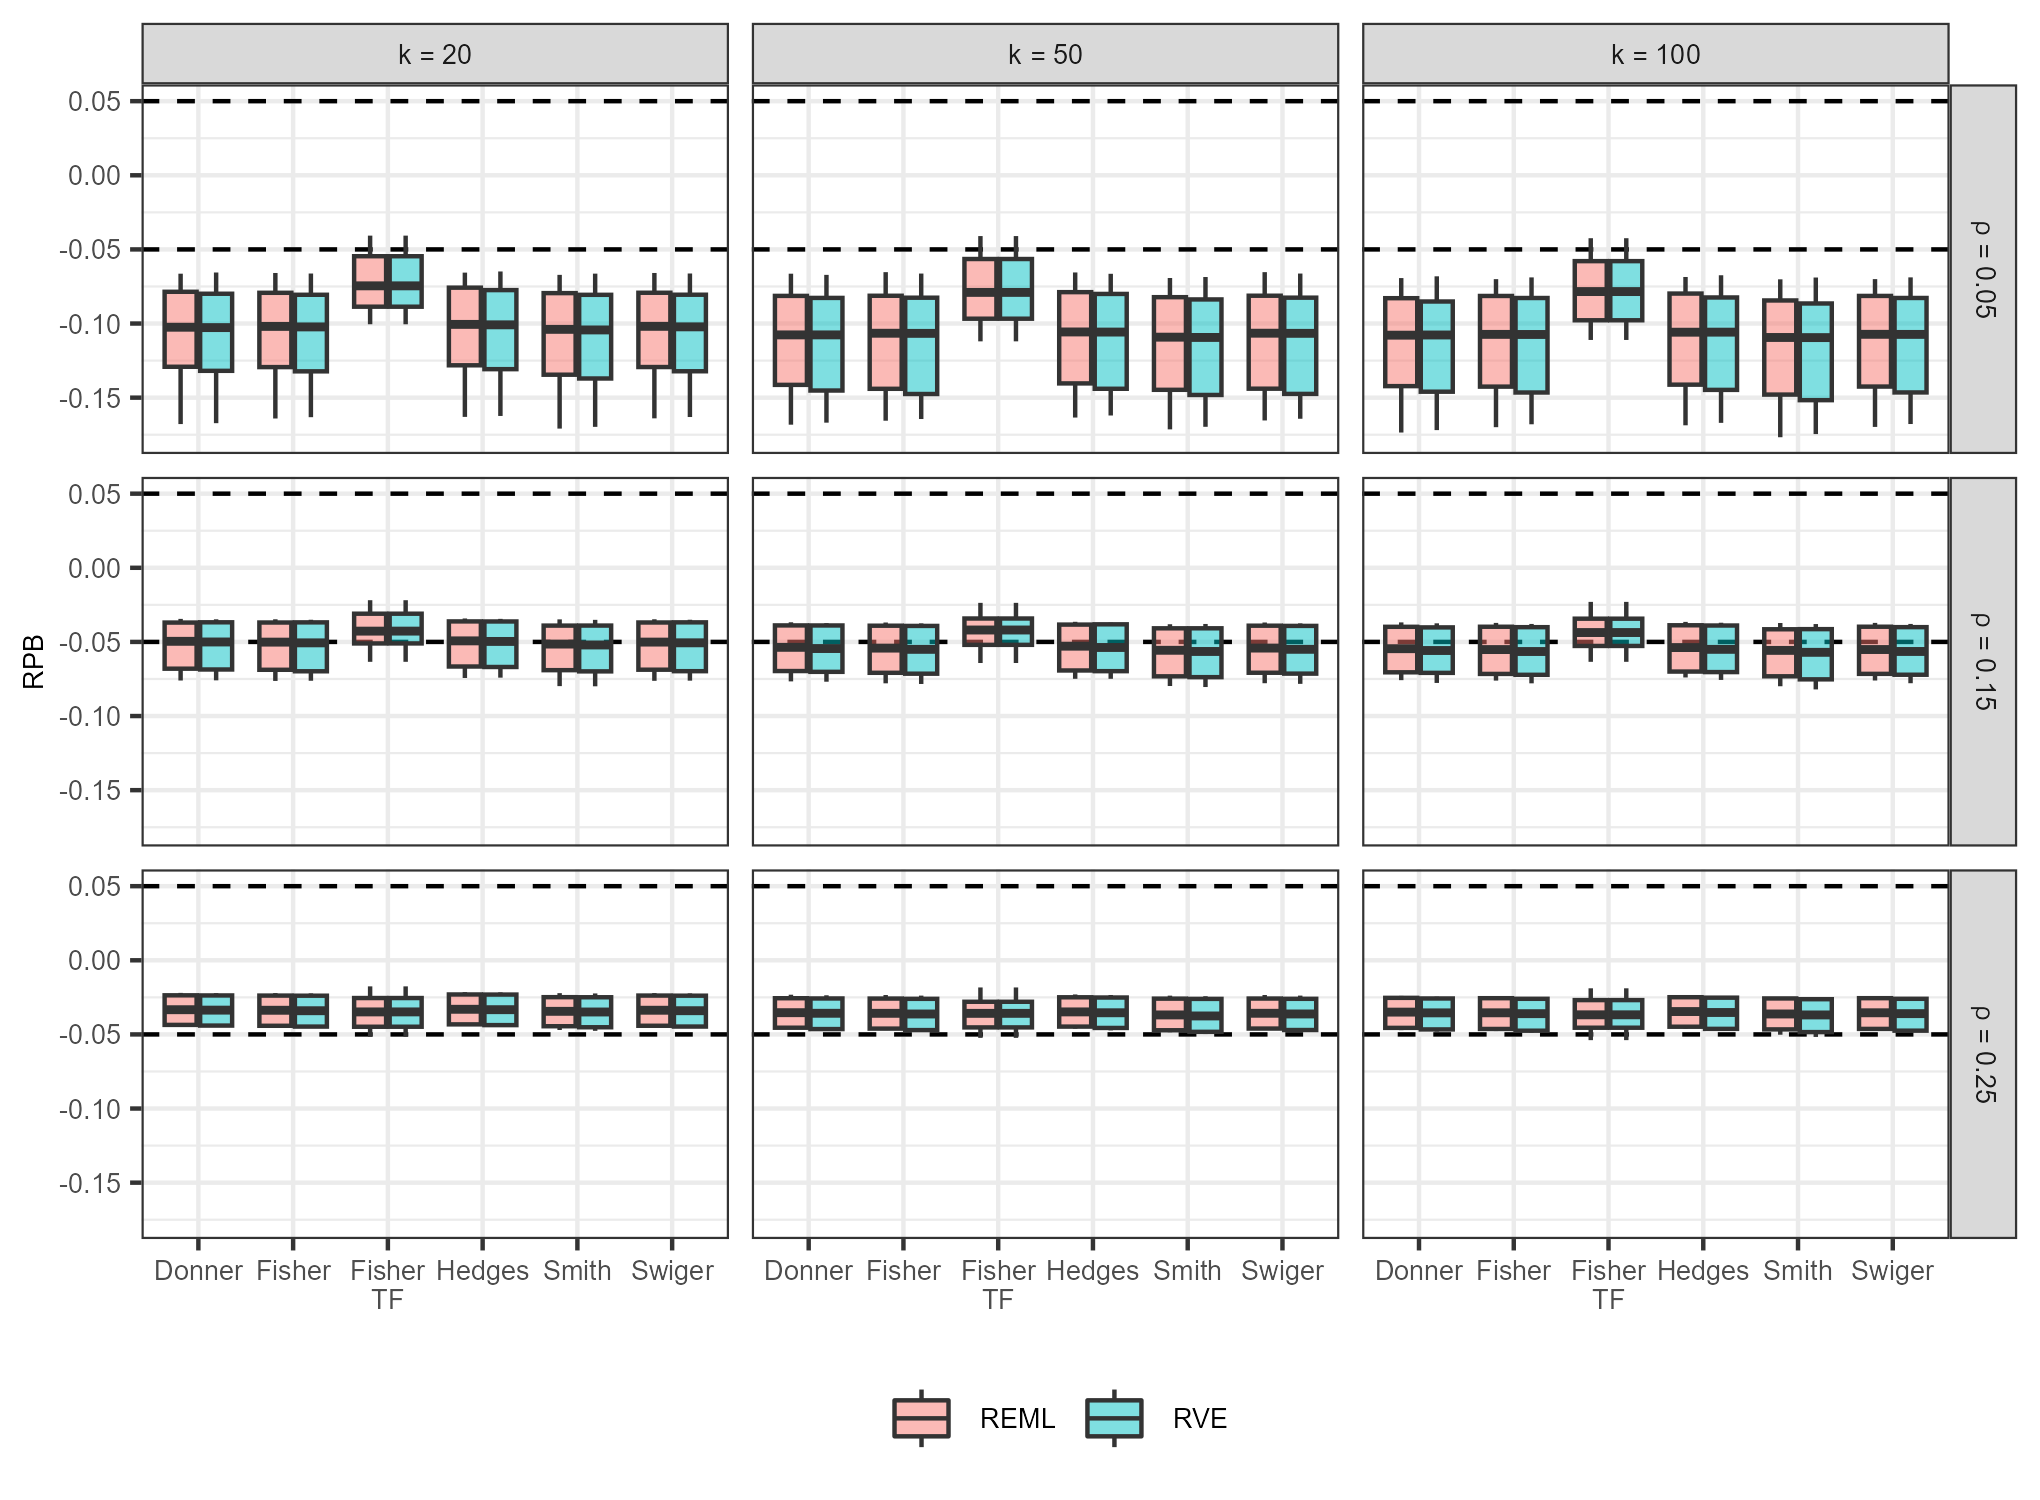
\includegraphics{Main/RPB_numICC.png}}
    \caption{The RPB of the pooled ICC estimates by the method of pooling, number of ICC estimates pooled ($k$) and the generating true ICC ($\rho$). \label{fig:RPBk}}
\end{figure*}

Figure \ref{fig:RPBtau} displays the RPB estimates as a function of between-study heterogeneity ($\tau$) and the true generating ICC values ($\rho$). There were very small differences in the degree of between-study heterogeneity that we evaluated. Higher between-study heterogeneity when the true generating ICC values are small ($\rho = .05$)resulted in negatively biased estimates across all methods with the Fisher TF variance formula resulting in the least biased estimates. For the $\rho$ values of 0.15, the estimates were very close to lacking substantial bias and no substantial bias was found when $\rho$ was generated using a value of 0.25. All the variance formulae underestimated the overall pooled effect. 
\begin{figure*}[h!]
\centerline{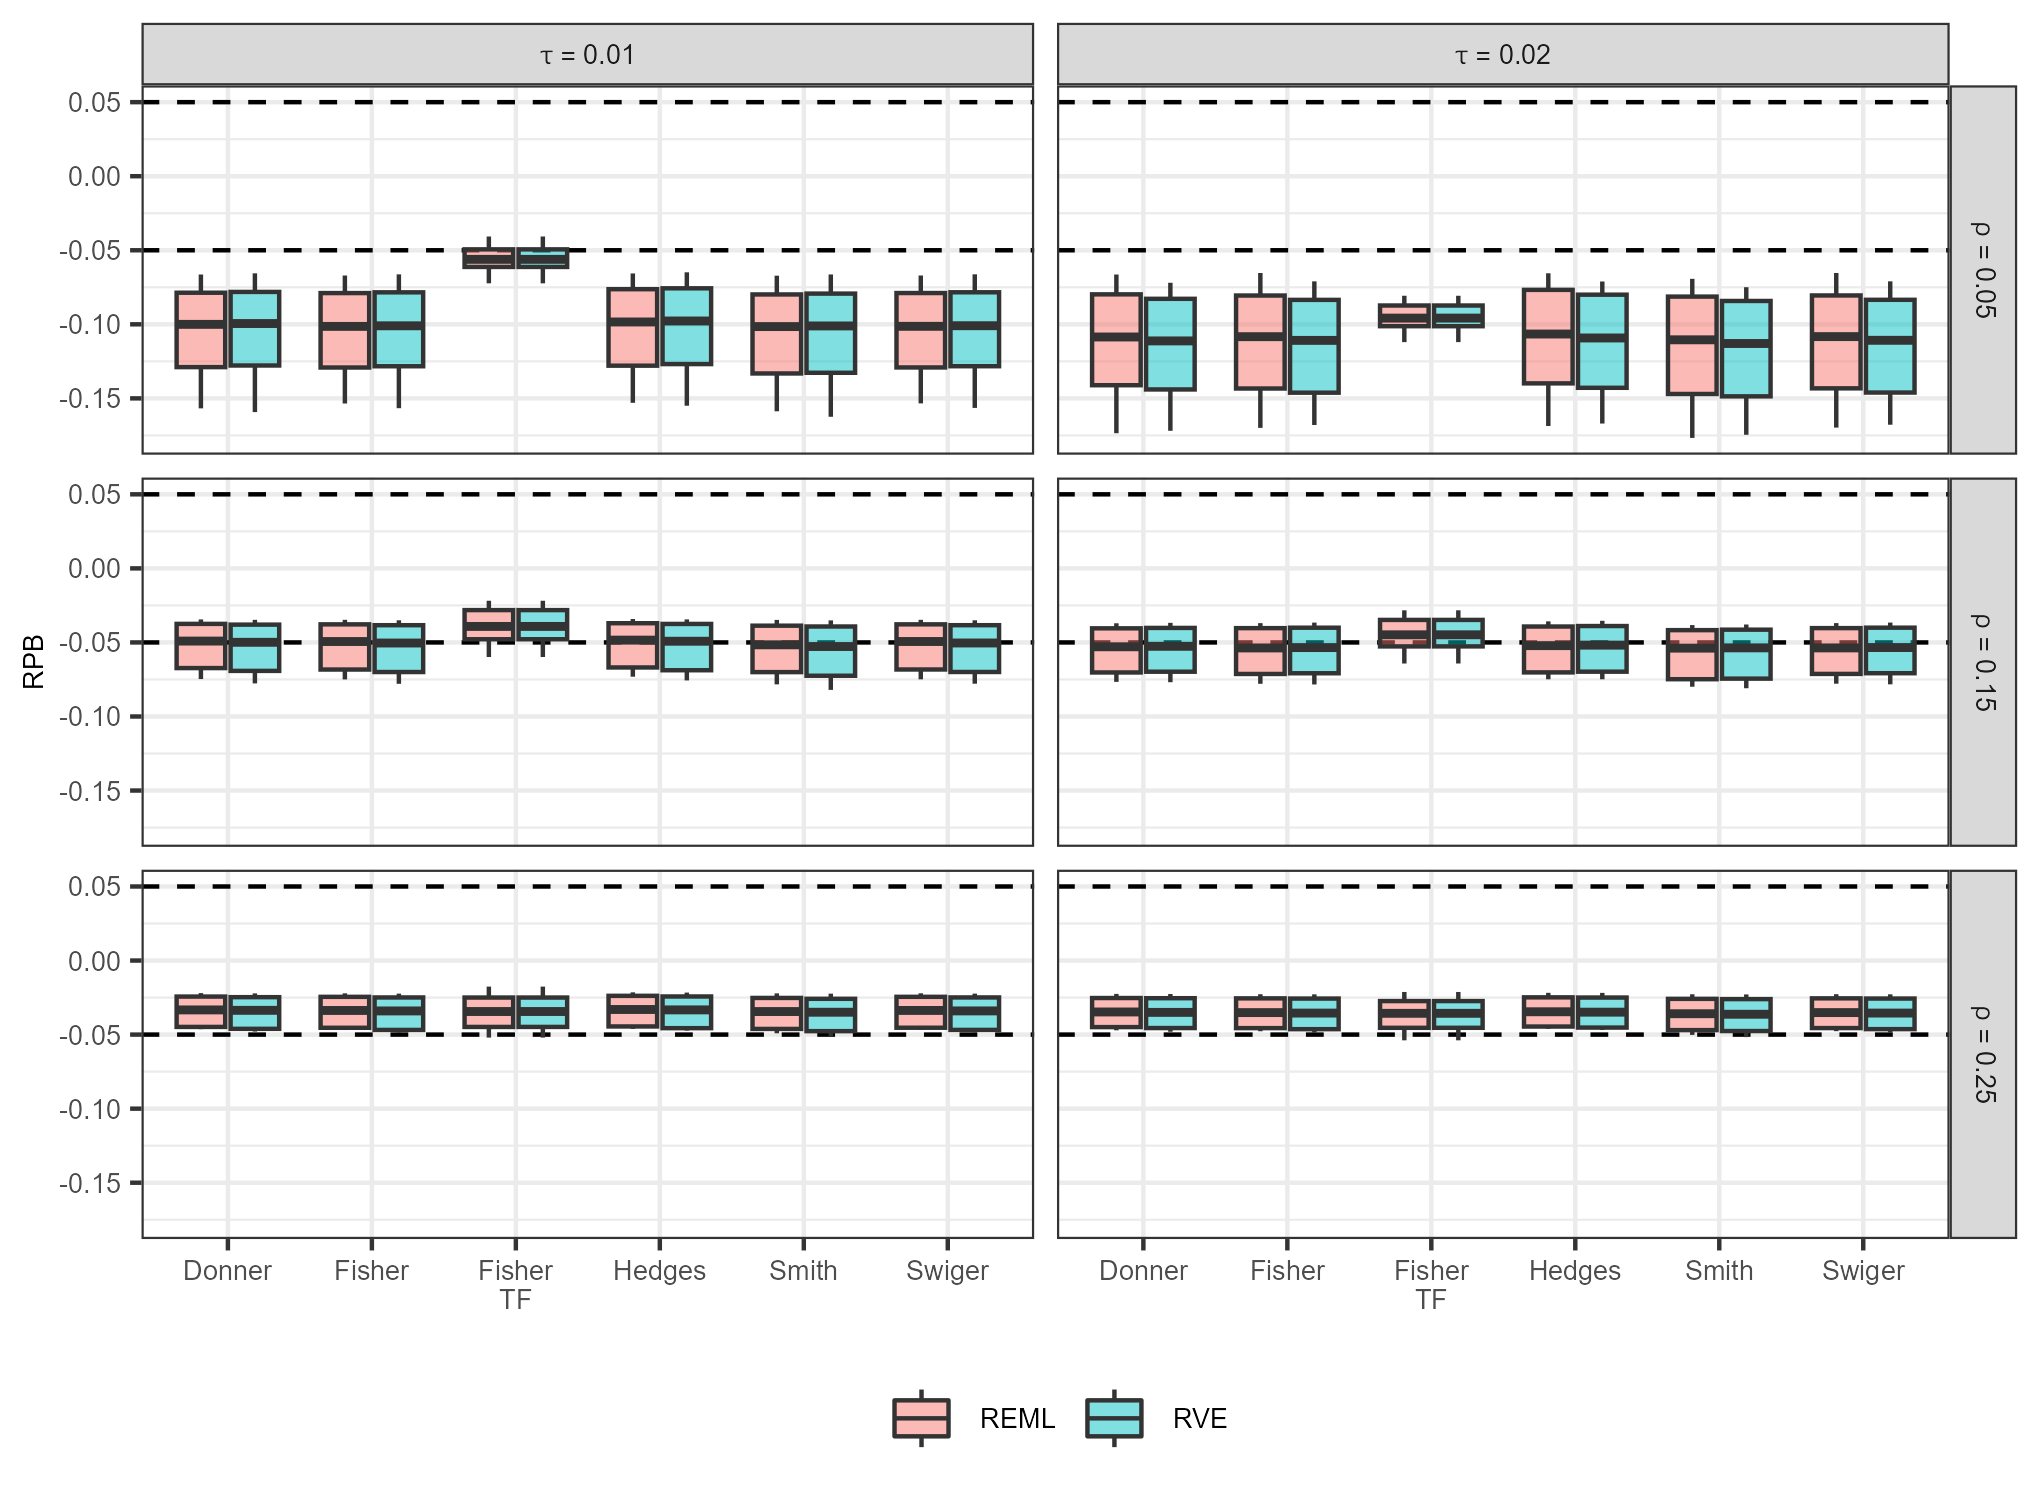
\includegraphics{Main/RPB_tau.png}}
\caption{The RPB of the pooled ICC estimates by the method of pooling, between study heterogeneity ($\tau$) and the generating true ICC ($\rho$). \label{fig:RPBtau}}
\end{figure*}

Figure \ref{fig:RMSEk} provides the results for the RMSE of the pooled ICC estimate as a function of number of estimates being pooled ($k$) and the true generating ICC values ($\rho$). Consistent with the RPB results, the Fisher TF variance formula results in the lowest RMSE for small true generating ICC values ($\rho=0.05$ and $\rho=0.15$).
\begin{figure*}[h!]
\centerline{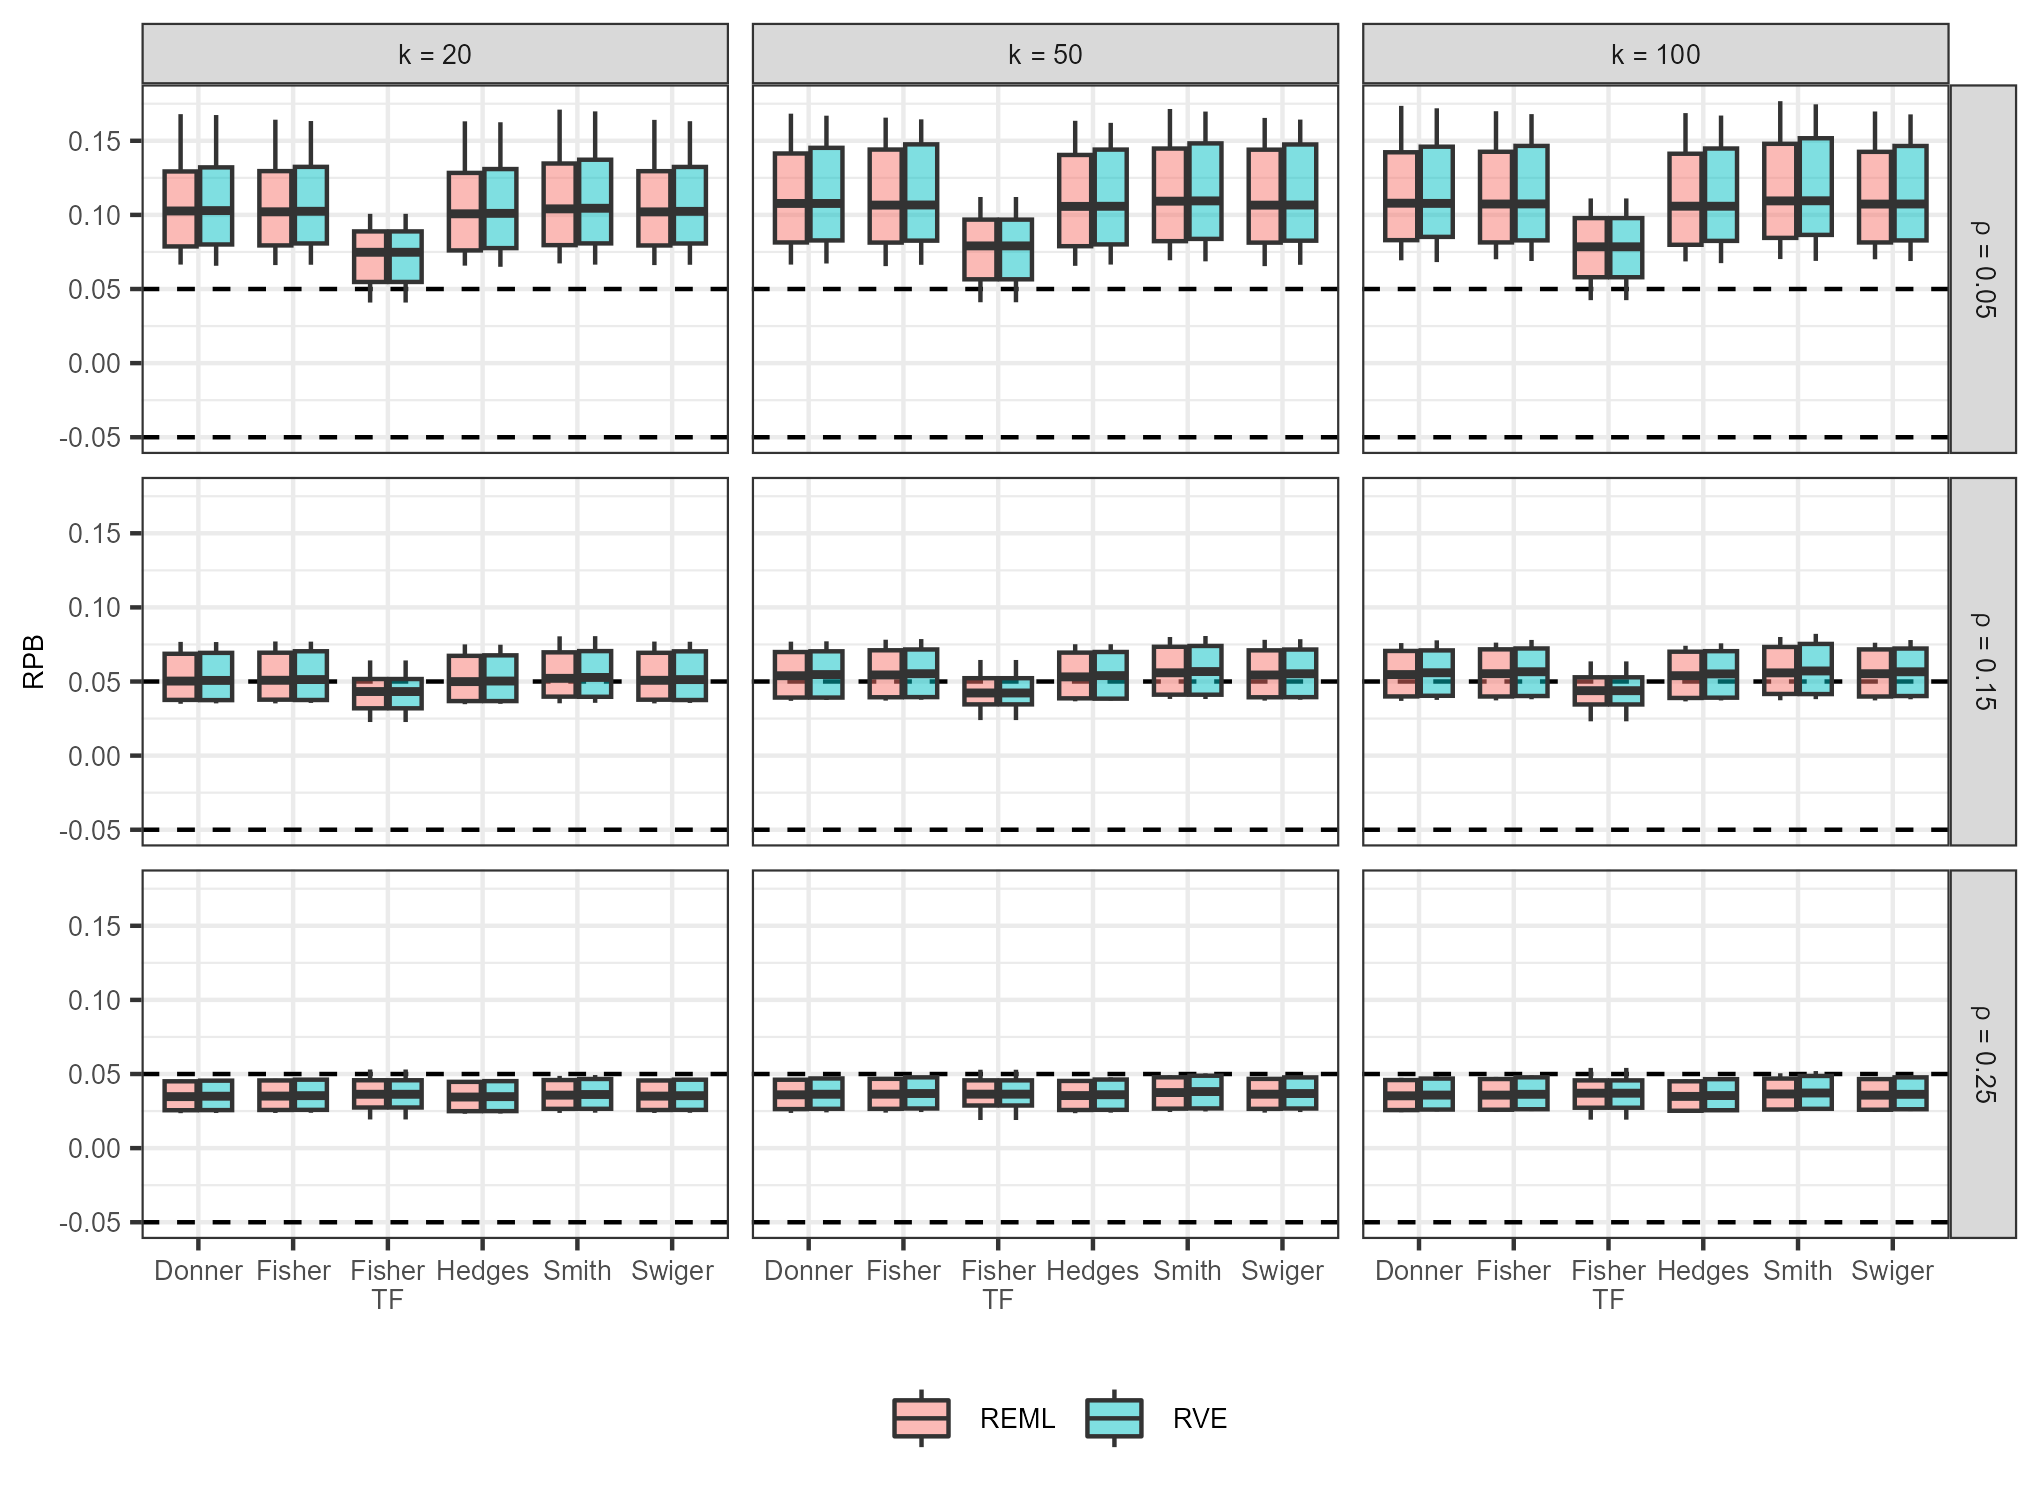
\includegraphics{Main/RMSE_numICC.png}}
    \caption{The RMSE using of the pooled ICC estimates by the method of pooling, number of ICC estimates pooled ($k$) and the generating true ICC ($\rho$).\label{fig:RMSEk} }
\end{figure*}


Figure \ref{fig:RMSEtau} contains the results for the RMSE of the pooled ICC estimate as a function of between-study heterogeneity ($\tau$) and the true generating ICC values ($\rho$). 

\begin{figure*}[h!]
\centerline{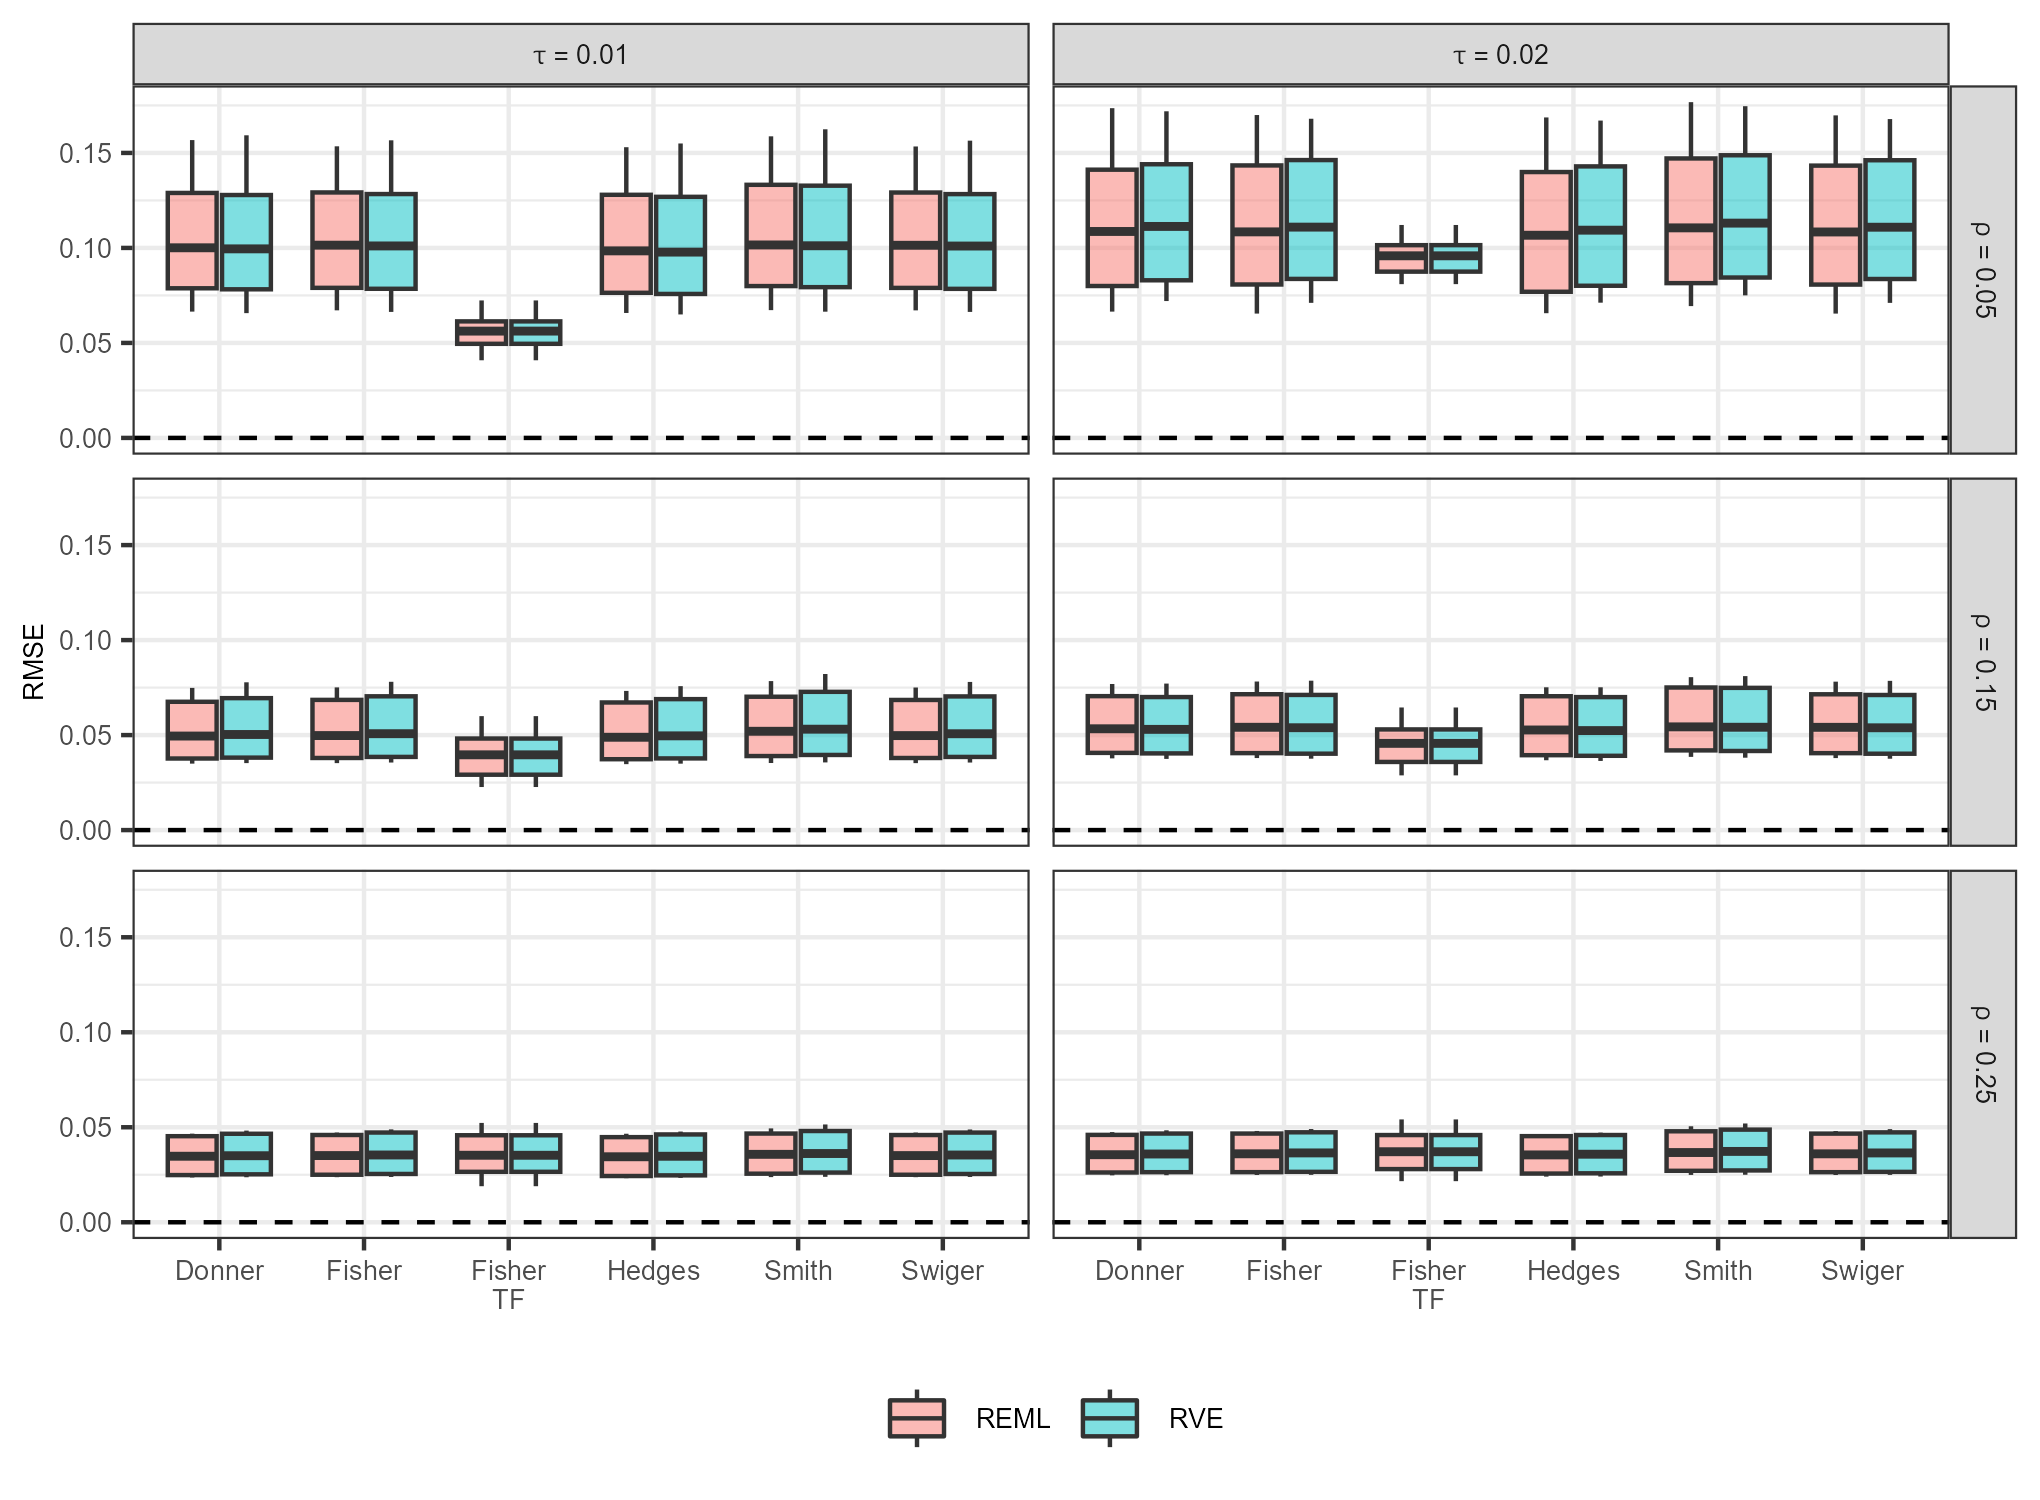
\includegraphics{Main/RMSE_tau.png}}
    \caption{The RMSE of the pooled ICC estimates by the method of pooling, between study heterogeneity ($\tau$) and the generating true ICC ($\rho$). \label{fig:RMSEtau} }
\end{figure*}


%%%%%%%%%%%%%%%%%%%%%%%%%%%%%%%%%%%%%%%

\subsubsection{SE of the Pooled ICC Estimate}




Figure \ref{fig:RPBkse_k} displays results for the RSEB of the pooled ICC estimate as a function of number of estimates being pooled ($k$) and the true generating ICC values ($\rho$). In addition, the number of ICC estimates pooled does not make a difference in RSEB across the conditions we evaluated. These results were consistent with other conditions we evaluated  (results in Supplementary Materials). 



\begin{figure*}[h!]
\centerline{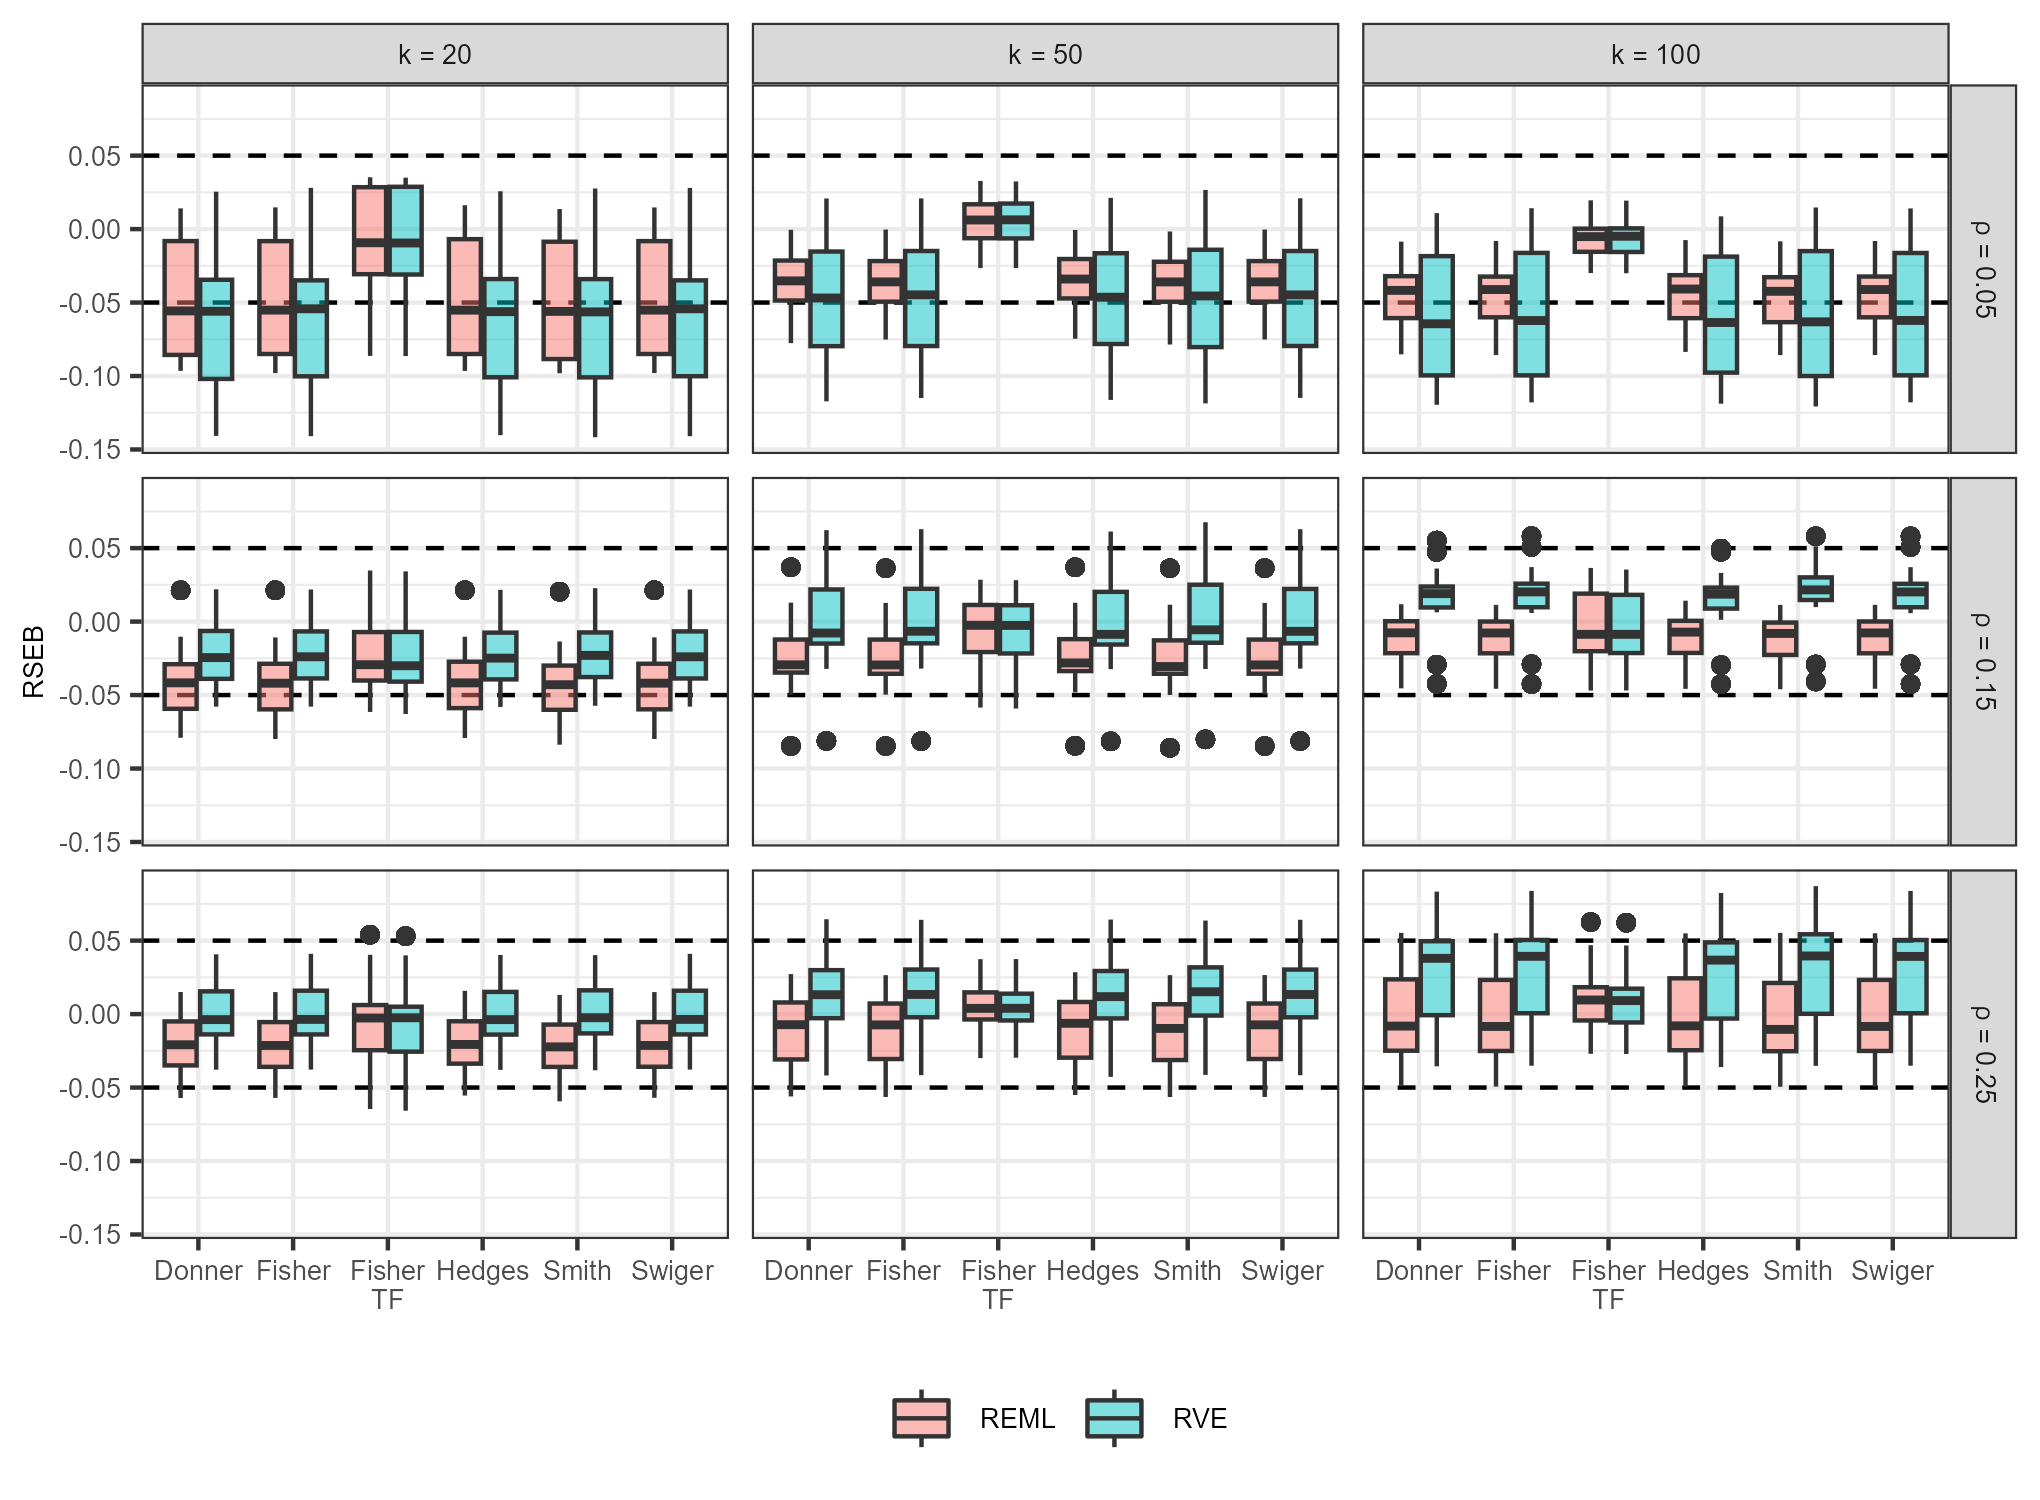
\includegraphics{Main/RSE_numICC.png}}
    \caption{The RSEB of the pooled ICC estimates by the method of pooling, number of ICC estimates pooled ($k$) and the generating true ICC ($\rho$). \label{fig:RPBkse_k}}
\end{figure*}




%%%%%%%%%%%%%%%%%%%%%%%%%%%%%%%%%%%%%%%%%%%%


\subsubsection{ Level 2 Variance of Primary Studies}


\paragraph{Relative parameter bias}

The Figures below display results for the RPB of the L2 variance. Figure \ref{fig:RPB_L2_tau} below provides a box plot of level-2 variances estimates by between-study heterogeneity. As can be seen in the Figure, for $\tau = 0.02$ and $\rho = 0.05$, the level-2 variance estimates were slightly biased when the generating true ICC was small ($\rho = 0.05$). We also wanted to confirm that the level-2 variance of the primary study was recovered well across the number of clusters condition. As can be seen in Figure \ref{fig:RPB_L2_j_mean} when we drew the number of clusters from a $U(30, 50)$ and when $\rho = 0.05$ this resulted in slightly biased estimates of the level-2 variance. Otherwise, across conditions, estimation of the level-2 variance was not substantially biased.

\begin{figure*}[h!]
\centerline{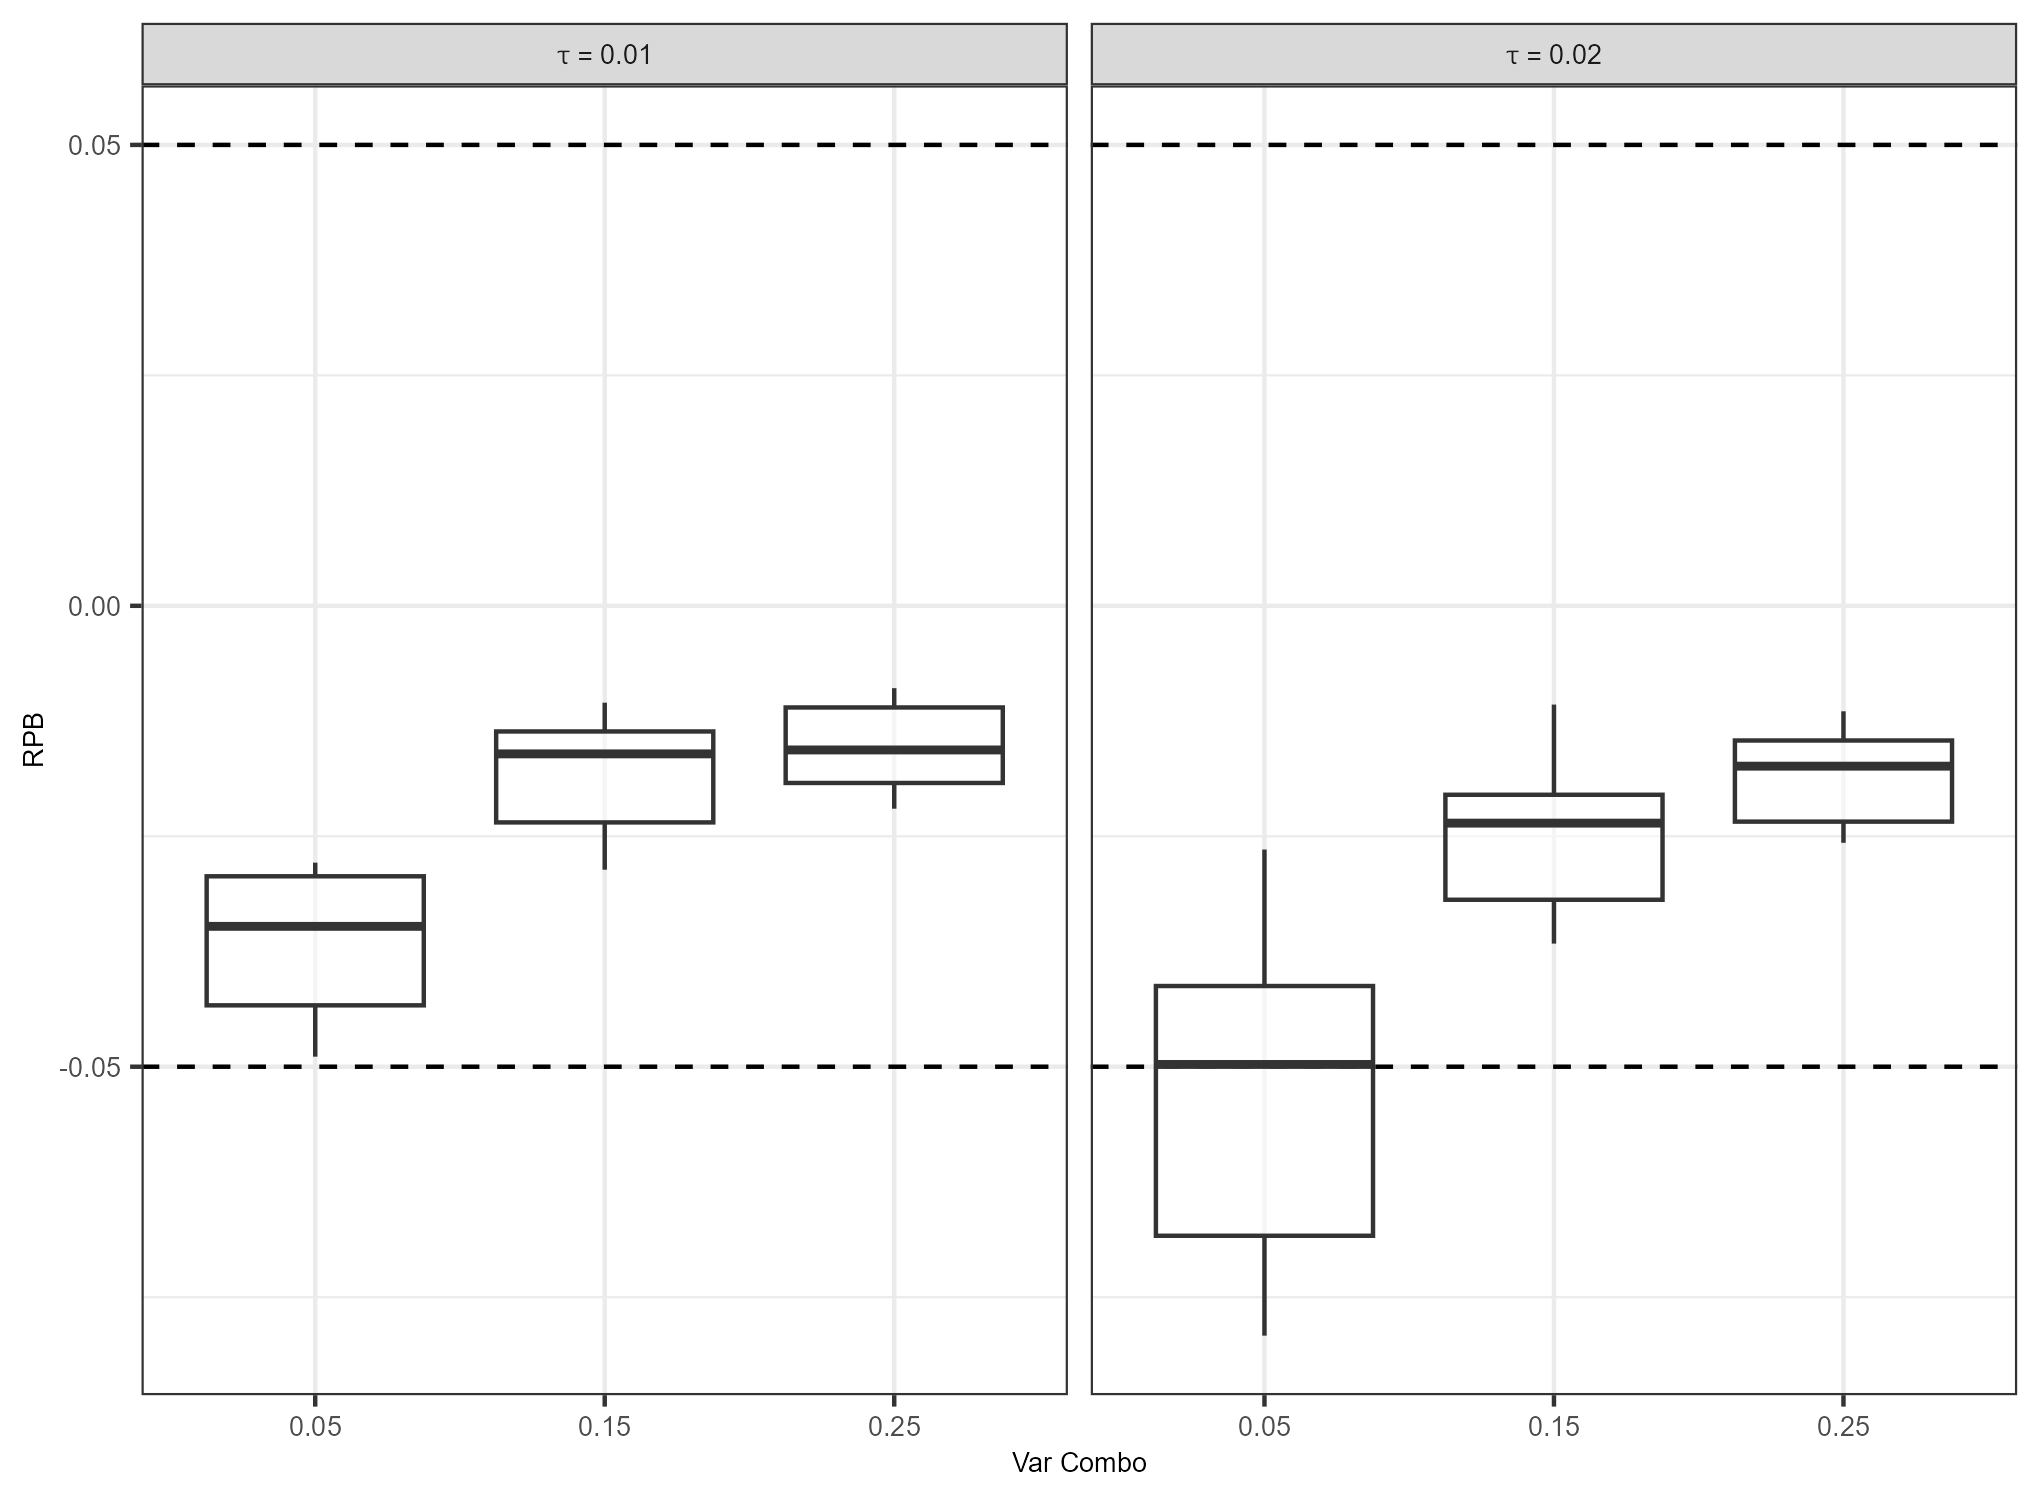
\includegraphics{Main/RPB_L2_tau_mean.png}}
    \caption{The RPB of the level-2 variance estimate by between study heterogeneity ($\tau$).\label{fig:RPB_L2_tau}}
\end{figure*}



\begin{figure}[h!]
\centerline{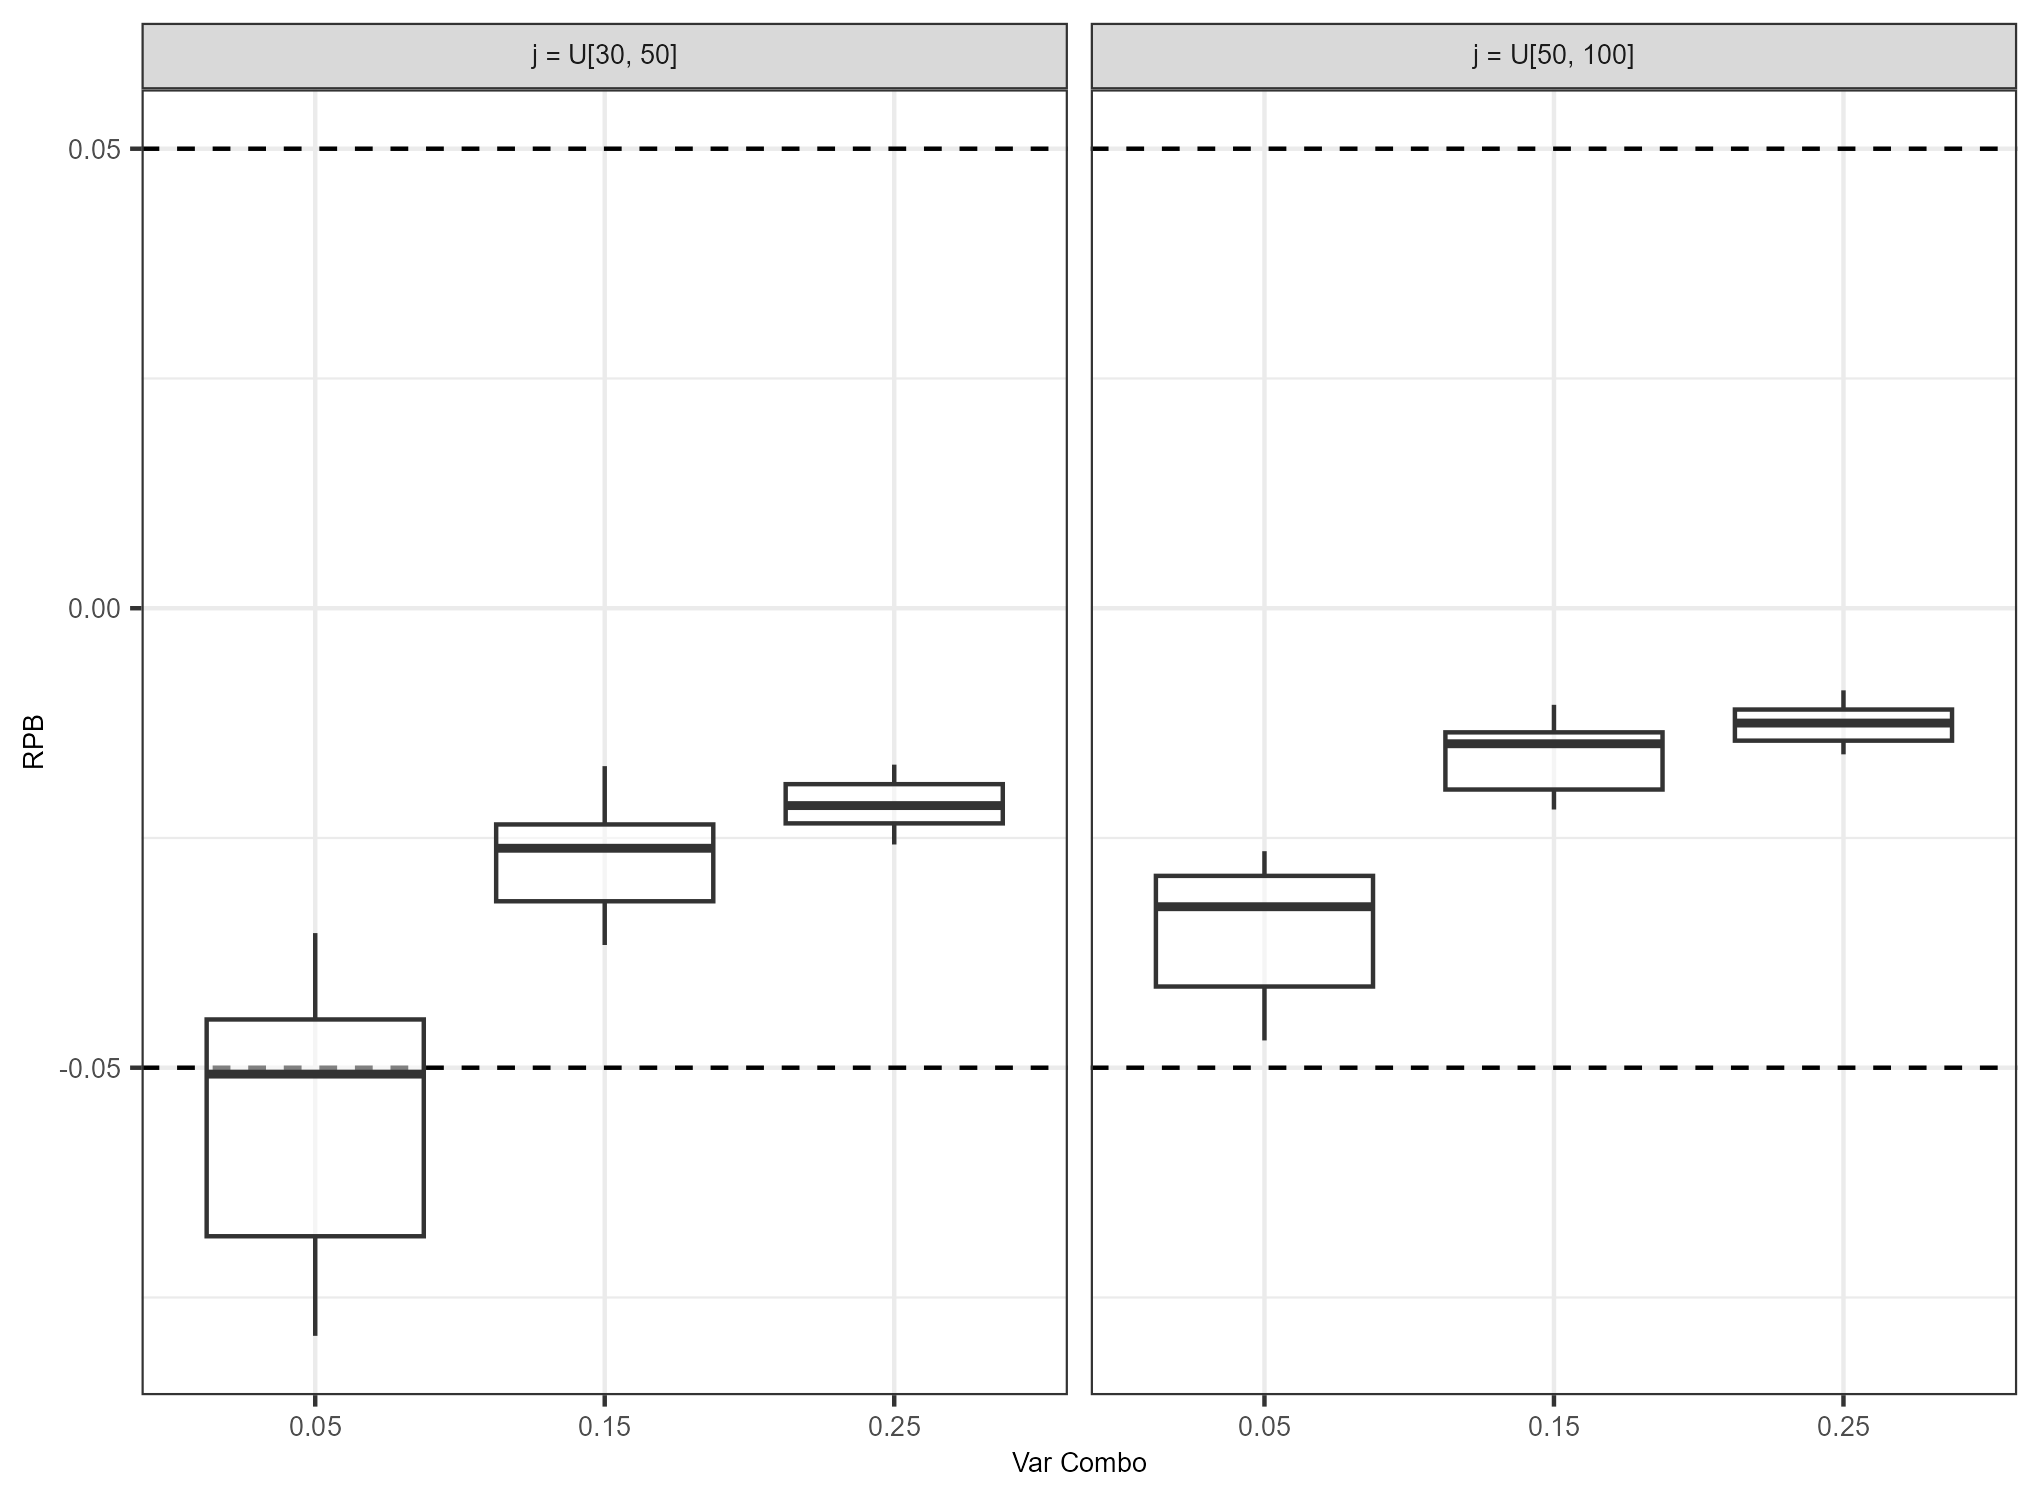
\includegraphics{Main/RPB_L2_j_mean.png}}
    \caption{The RPB of the level-2 variance estimate by number of clusters ($\tau$).\label{fig:RPB_L2_j_mean}}
\end{figure}




\section{Discussion}
There is a need for using accurate ICC values for a priori power analyses or meta-analyses of effect sizes in clustered data scenarios. The most frequently used methods for imputing ICC estimates in these scenarios can result in inaccurate values that ultimately negatively impact the inferences resulting from the associated analyses in which the values are used. Little research has focused on how best to capture reasonable ICC values to improve the validity of associated inferences. Meta-analytic pooling of relevant observed ICC values offers a principled method for imputing ICC values. However, there has not been a lot of research exploring how best to meta-analyze ICC estimates. The unknown shape of the sampling distribution of ICC estimates offers a particular challenge to the meta-analytic pooling of ICC estimates. In addition, the formulation for the variance of the sampling distribution of ICC estimates is unknown although several methodological researchers have suggested various formulas \cite{fisherTheoryStatisticalEstimation1925, hedgesVarianceIntraclassCorrelations2012, donner1980a, smith1957, swiger1964, fisher1970statistical}. The current study compares some of the variance formulas (used in the weighting of ICCs when they are pooled) and compares two methods for meta-analytic pooling (REML versus RVE) across a number of design conditions. Ultimately, this study is intended to assess the meta-analytic pooling of ICC to inform researchers about the best way to do so.  

The results of this study provide some guidelines for applied researchers when (1) they need to impute ICC values for use in an a priori power analysis for clustered data, or (2) the researcher is conducting a meta-analysis that contains effect sizes for clustered data in any of the primary studies in the meta-analytic dataset that need to be corrected for clustering and that might be missing associated ICC estimates, or (3) the researcher is meta-analyzing ICC estimates. The results suggest that, for the design conditions we examined, there were no huge differences in the pooled ICC estimates when using REML versus using RVE to pool ICC estimates. Therefore, when meta-analyzing ICCs in the kinds of scenarios that we examined, REML and RVE appear to function equivalently. There were not huge differences among variance formulae, but the Fisher TF formula (Equation \ref{fisher_transformed_ICC_var}; \citeA{fisher1970statistical}) performed best across the performance criteria we assessed and the design conditions we tested. The Fisher TF formula provided the least biased pooled ICC estimates and SE of the ICC estimates for the $\rho=0.05$ conditions, and it was the only $v_r$ formula without substantial bias in the pooled ICC estimates in the $\rho = 0.15$ conditions.  So, we recommend using the Fisher TF formula for the ICC variance for use in the inverse variance weights when pooling ICC estimates. For large $\rho$ values ($\rho=0.25$), no bias was found as a function of the $v_r$ formula used. 

Regarding primary study characteristics, larger sample sizes resulted in less biased pooled ICC estimates across all $v_r$ formulae. Last, we did not find any distinctive impact on ICC estimation of the number of ICC estimates being pooled (k= 20, 50, versus 100). Future studies could evaluate how well pooling fewer ICC estimates captures the true ICC parameter value.  

Finally, these meta-analytic pooling ICC estimates methods are relatively accessible to applied researchers. For example, RVE for meta-analysis is available in software like Stata, SPSS, and R. These pooling methods are already being used widely by applied meta-analysts. We provide sample code that also facilitates the calculation of the ICC variance using several of the options in our supplementary materials. We also provide the code for meta-analysis of ICC estimates.



We only estimated variance components of the primary studies in each simulated meta-analysis using REML. However, researchers use a variety of estimation methods when estimating variance components and will not always report which method they implemented. As stated before, estimating variance components accurately is essential for getting accurate ICC estimates (see Equation \ref{ICC_algebra}), so pooled estimates will only be as accurate as the ICC estimates that are being pooled. Future studies might investigate the impact of various estimation methods for the variance components themselves on which each ICC estimate is based. 
    
We also investigated scenarios in which each primary study only reported a single ICC estimate. The reality is that studies often report results for multiple outcomes, and therefore, multiple ICC values might be available per primary study. These outcomes may be related and so will be the resulting ICC estimates. The researcher might want to include all the ICC estimates reported for the related outcomes when pooling ICC estimates. Luckily, RVE is typically used to account for dependence in meta-analytic data sets, so this method should be robust to this limitation. The work accomplished in this study could be extended to evaluate methods for pooling of ICC estimates in scenarios with within-study dependence in the ICCs.  

There are several limitations to the variance formulae derived for an ICC estimate for reasonable use in meta-analysis of ICC estimates. The formulae derived by \citeA{donner1980a} and \citeA{smith1957} both require knowledge of how many individuals there are per cluster in a primary study. However, typically primary studies do not report how many individuals there are per cluster.  Also, the $v_r$ formula derived by \citeA{hedgesVarianceIntraclassCorrelations2012} requires knowledge of the variance of the cluster-level variance in a primary study. This is also not often reported in primary studies which drastically limits a researcher ability to use this formula unless they have access to the primary study's raw data. Furthermore, some of the formulae require the weighted mean cluster size \cite{smith1957, swiger1964} instead of the arithmetic mean cluster size. However, it is not likely that primary studies will report the weighted mean cluster size nor be clear about how the average cluster size was calculated if it is reported. Further research is needed to evaluate the use of the mean versus a weighted mean cluster size in the relevant variance formulae. 

Furthermore, we only evaluated pooling of ICC estimates for ICCs for two-level data. While in educational, and social science research more generally, three-level data are also commonly analyzed. Future research, could evaluate use of these methods with three-level data. Only \cite{hedgesVarianceIntraclassCorrelations2012} has derived a formula for the variance of an ICC for clustered data with three levels of nesting. 

In summary, we recommend not summarizing across ICCs that come from samples that are too different. The additional obstacle of including ICCs from studies that are capturing variability in outcomes that deviate too much from the primary construct of interest is a further threat to the validity of the resulting inferences due to generalizability error. In addition, researchers are cautioned against use of ICCs when they are based on a sample from a population that is too different than the population that is the focus of the relevant analysis (meta-analysis of effect sizes or power analyses for clustered data) \cite{jacob2010}. However, under the conditions we evaluated, it seems reasonable to use Fisher's $v_r$ with RVE or REML to pool ICC estimates, rather than relying on the more ad hoc methods that are typically used for imputing values.


\bibliography{Main/QP.bib}

%\renewcommand{\bibname}{References}
%\printbibliography



\end{document}
